\documentclass[11pt]{ama-article}
\usepackage{tikz}
\usetikzlibrary{arrows.meta,positioning,calc,shapes.geometric,decorations.pathreplacing}
\setcounter{MaxMatrixCols}{13}
\accroche{Here's AMA}
\siterevue{academiedesmathsappliquees.com}
\urlrevue{http://academiedesmathsappliquees.com/}
\fichierlogo{logo-ama}
\anneeparution{2026}
\issn{2960-1234/\$}
\doi{10.5281/ama.2026.0031}
\droits{Tous droits réservés.}
\titre{Distribuer l'eau équitablement dans un quartier quand la demande est incertaine}
\titrecourt{Distribution équitable de l'eau sous incertitude}
\auteur[*]{Narcisse ATTIOU}{a}{narcisse.attiou@ama.edu}
\auteur{Aïchatou TRAORÉ}{a}{aichatou.traore@ama.edu}
\auteur{Omotola AFOUDA}{a}{omotola.afouda@ama.edu}
\auteur{Godwin AKAKPO}{a}{godwin.akakpo@ama.edu}
\auteur{Mathilde Sena Phasiline GUEDENON}{a}{mathilde.guedenon@ama.edu}
\auteur{Clemou Pakychel Désir MOUSSOUNOU}{a}{clemou.moussounou@ama.edu}
\auteurcourt{N. ATTIOU et al.}
\affiliation{a}{Académie des Mathématiques Appliquées, Cotonou, Bénin}
\adressecorrespondance{Académie des Mathématiques Appliquées, Cotonou, Bénin.}
\motscles{réseau d'eau\\ optimisation quadratique\\ descente de gradient\\ incertitude\\ graphe orienté}
\encadrant{Ir. Charbel Mamlankou}
\module{Mathématiques fondamentales pour l'IA -- Thème 3}
\niveau{2\textsuperscript{e} année}
\anneeacademique{2025--2026}

\definecolor{reservoirgreen}{RGB}{65,150,75}
\definecolor{neighborhoodblue}{RGB}{70,130,200}
\definecolor{criticalred}{RGB}{210,45,45}
\definecolor{edgegray}{RGB}{70,70,70}
\tikzset{quartier/.style={circle,draw=black,fill=neighborhoodblue!35,minimum size=1cm},
  reservoir/.style={rectangle,draw=black,fill=reservoirgreen!75,minimum width=1.25cm,minimum height=1.25cm},
  conduit/.style={draw=edgegray,line width=1.1pt,-{Latex[length=2.2mm]}},
  connexion/.style={draw=black!75,line width=1.1pt,-{Latex[length=2.2mm]}},
  boucle/.style={draw=black!60,line width=1.1pt,-{Latex[length=2.2mm]}},
    pont/.style={draw=criticalred,line width=1.5pt,dashed,-{Latex[length=2.2mm]}},
    edge-label/.style={fill=white,inner sep=1.5pt,font=\scriptsize,midway}}
\resume{Ce travail étudie la répartition équitable de l'eau dans un réseau de conduites lorsque la demande des quartiers est incertaine. Le réseau est modélisé par un graphe orienté et une matrice d'incidence, tandis que les demandes sont représentées par des variables gaussiennes. Nous formulons une optimisation quadratique pénalisant la violation de la conservation des flux et imposons la positivité des débits par projection. La solution est calculée par descente de gradient projetée, puis évaluée sur six expériences numériques et 1000 scénarios Monte-Carlo. Dans le protocole étudié, la stratégie optimisée réduit le coût technique moyen de 4,83\,\% par rapport à la distribution proportionnelle, avec une baisse de la violation moyenne de 13,527 à 3,117.}
\abstract{This work studies equitable water allocation in a pipe network when district demand is uncertain. The network is modeled by a directed graph and an incidence matrix. We formulate a quadratic optimization problem and solve it with projected gradient descent. Six numerical experiments and 1,000 Monte Carlo scenarios show a 4.83\% reduction in mean technical cost compared with proportional allocation.}
\begin{document}
\maketitle

\section{Introduction}

Une société de distribution d'eau alimente plusieurs quartiers d'une ville à partir de
quelques réservoirs, reliés entre eux par un réseau de conduites dont le débit n'est pas
illimité. Aujourd'hui, la répartition de l'eau entre les quartiers se fait de façon empirique,
proportionnellement à la demande historique, sans réelle optimisation. Cette pratique pose
deux problèmes distincts : d'une part, rien ne garantit qu'elle minimise le coût global
d'acheminement de l'eau à travers le réseau ; d'autre part, la demande réelle de chaque
quartier n'est jamais connue à l'avance avec certitude et varie de façon imprévisible d'un
jour à l'autre.

L'objectif de ce projet est de construire un outil qui calcule une répartition de l'eau à la
fois plus équitable et moins coûteuse que la pratique actuelle, tout en restant fiable
lorsque la demande réelle s'écarte des prévisions. Le travail se déroule en deux volets
complémentaires, imposés par le cadrage du sujet~\cite{sujets-ama} :

\begin{itemize}[leftmargin=*]
    \item un \textbf{rapport} qui pose le problème en mathématiques, démontre les résultats
    à la main, et non seulement de façon numérique, puis confronte ces résultats à des
    expériences ;
    \item un \textbf{outil informatique}, livré séparément du rapport, qui prend en entrée la
    description d'un réseau et d'une demande, et qui produit une comparaison chiffrée entre
    l'ancienne méthode et la nouvelle.
\end{itemize}

Le fil conducteur du projet suit le pipeline méthodologique imposé :
partant d'un problème réel, on formule une question de recherche, on pose des hypothèses et des
variables, on construit un modèle mathématique qui mobilise conjointement l'algèbre linéaire,
les probabilités et statistiques, et les mathématiques discrètes, avant de traduire ce modèle
en un problème d'optimisation résolu par descente de gradient, puis validé numériquement.

Le présent document rassemble la topologie du réseau, sa représentation algébrique, le modèle
probabiliste et la formulation d'optimisation, puis confronte ces résultats aux sorties
numériques effectivement produites. Les six expériences sont documentées avec leurs tableaux
et figures ; les expériences 1 et 2 ajoutent la comparaison à la stratégie de référence et son
extension à 1000 scénarios Monte-Carlo.


\section{Formulation du problème}
\label{sec:formulation}


\subsection{Entrées et sorties du problème}

\begin{table}[h!]
\centering
\begin{tabular}{>{\raggedright\arraybackslash}p{7cm}>{\raggedright\arraybackslash}p{7cm}}
\toprule
\textbf{Entrées} & \textbf{Sorties attendues} \\
\midrule
Topologie du réseau : réservoirs, quartiers, conduites &
Un vecteur de débits optimal $q^\star$ sur chaque conduite \\
Capacités des conduites et coût unitaire $c_e$ de chacune &
Une comparaison chiffrée entre la distribution actuelle et $q^\star$, sur plusieurs scénarios simulés \\
Paramètres de la loi de demande de chaque quartier, $\mu_i,\sigma_i$ &
Une caractérisation de la robustesse de $q^\star$ face à l'incertitude \\
Offre totale disponible aux réservoirs & \\
\bottomrule
\end{tabular}
\caption{Entrées et sorties du problème}
\end{table}

\subsection{Hypothèses de modélisation}

Deux hypothèses sont imposées par le cadrage du sujet et ne sont pas remises en cause par le
groupe : la demande de chaque quartier est une variable aléatoire gaussienne
$D_i \sim \mathcal{N}(\mu_i,\sigma_i^2)$, et la contrainte d'égalité $Aq=b$ doit être traitée
par pénalisation (jamais par multiplicateurs de Lagrange), tandis que la contrainte
$q\ge 0$ est traitée par projection.

Le groupe a, de son côté, fixé les éléments suivants, détaillés à la Section~\ref{sec:graphe} :
le nombre de quartiers et de réservoirs (8 quartiers, 2 réservoirs), la topologie précise du
graphe, les valeurs de $c_e$, $\mu_i$ et $\sigma_i$.

\subsection{Contraintes mathématiques et formulation}
\label{sec:formulation-math}

Le problème s'écrit comme un programme quadratique sous contraintes linéaires :
\begin{equation}
q^\star = \operatorname*{arg\,min}_{q} \sum_{e\in E} c_e\, q_e^2
\qquad \text{sous} \qquad Aq = b, \quad q \ge 0,
\label{eq:probleme-original}
\end{equation}
où $A$ est la matrice d'incidence du graphe orienté du réseau (Section~\ref{sec:algebre}), $q$
le vecteur des débits sur chaque conduite, et $b$ le vecteur rassemblant l'offre injectée aux
réservoirs et la demande à satisfaire à chaque quartier. La première contrainte traduit la
conservation des flux ; la seconde interdit un débit négatif sur une conduite dont
l'orientation de référence a été fixée par le Membre 1.

% =======================================================================
\section{Développement mathématique}
% =======================================================================

Conformément à la structure imposée pour le rapport, cette section couvre les cinq volets
exigés : structure discrète, représentation algébrique, modélisation probabiliste, analyse
statistique, et formulation d'optimisation avec dérivation complète du gradient.

% -----------------------------------------------------------------------
\subsection{Structure discrète : le graphe du réseau}
\label{sec:graphe}
% -----------------------------------------------------------------------

\subsubsection{Composition du réseau}

Le réseau est modélisé comme un graphe orienté connexe
\[
G = (V,E), \qquad V = V_R \cup V_Q,
\]
composé de $n=10$ nœuds et $m=13$ conduites. Les nœuds représentent les réservoirs et les
quartiers, tandis que les arêtes correspondent aux conduites qui les relient.

\begin{table}[h!]
\centering
\begin{tabular}{>{\raggedright\arraybackslash}p{3cm}
                >{\raggedright\arraybackslash}p{4cm}
                >{\raggedright\arraybackslash}p{7.3cm}}
\toprule
\textbf{Nœud} & \textbf{Type} & \textbf{Rôle} \\
\midrule
$R_1,R_2$ &
Réservoirs sources &
Injectent le débit dans le réseau. Le système est donc un réseau multi-sources. \\
$Q_1,\ldots,Q_8$ &
Quartiers de demande &
Consomment un débit incertain $D_i\sim\mathcal{N}(\mu_i,\sigma_i^2)$. Ce sont des nœuds de
transit pur, sans stockage. \\
\bottomrule
\end{tabular}
\caption{Composition du réseau}
\end{table}

Les conduites sont regroupées selon leur fonction :

\begin{table}[h!]
\centering
\begin{tabular}{>{\raggedright\arraybackslash}p{3.5cm}
                >{\raggedright\arraybackslash}p{6cm}
                >{\raggedright\arraybackslash}p{5cm}}
\toprule
\textbf{Groupe} & \textbf{Conduites} & \textbf{Fonction} \\
\midrule
Backbone $R_1$ &
$R_1\!-\!Q_1,\ R_1\!-\!Q_2,\ Q_2\!-\!Q_3,\ Q_3\!-\!Q_4$ &
Chaîne d'alimentation principale depuis $R_1$. \\
Backbone $R_2$ &
$R_2\!-\!Q_5,\ R_2\!-\!Q_6,\ Q_6\!-\!Q_7,\ Q_7\!-\!Q_8$ &
Chaîne d'alimentation principale depuis $R_2$. \\
Connexions inter-zones &
$Q_4\!-\!Q_5,\ Q_3\!-\!Q_6$ &
Relient les deux zones par deux chemins indépendants. \\
Boucles de redondance &
$Q_2\!-\!Q_4,\ Q_5\!-\!Q_6,\ Q_6\!-\!Q_8$ &
Offrent un second chemin à certains quartiers. \\
\bottomrule
\end{tabular}
\caption{Répartition fonctionnelle des conduites}
\end{table}

\subsubsection{Schéma du réseau}

La Figure~\ref{fig:topologie-reseau} représente la topologie retenue. Les carrés verts
représentent les réservoirs, les cercles bleus les quartiers, et les traits rouges pointillés
les conduites critiques identifiées comme des ponts.

\begin{figure}[p]
\centering
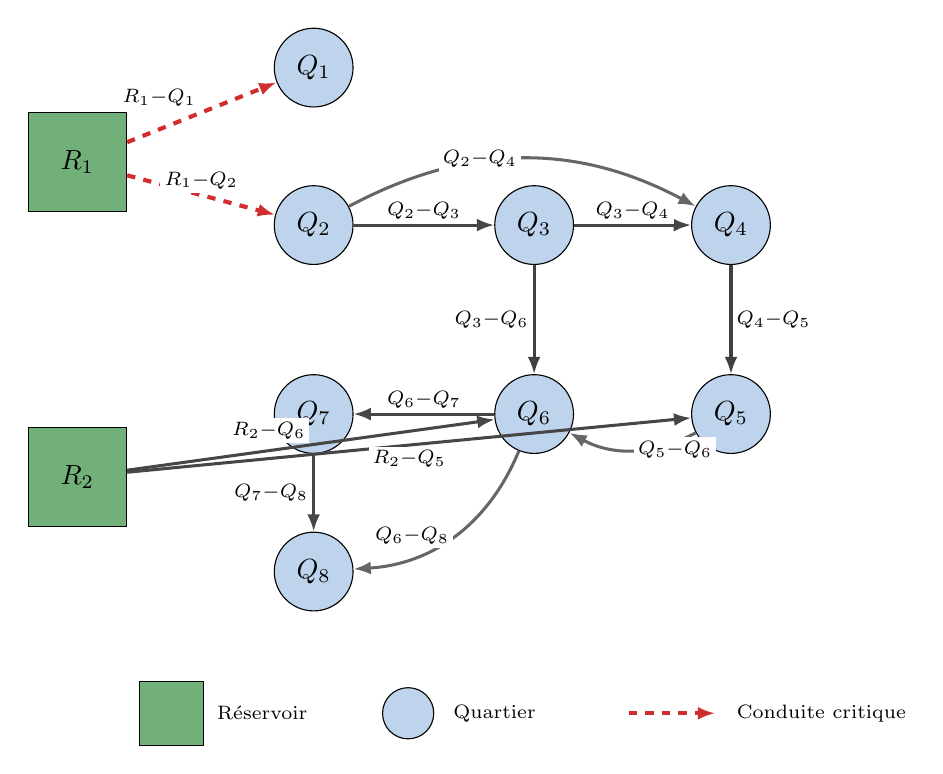
\begin{tikzpicture}[scale=1.0,transform shape,node distance=1.4cm and 1.8cm]

\node[reservoir] (R1) at (0,4) {$R_1$};
\node[reservoir] (R2) at (0,0) {$R_2$};

\node[quartier] (Q1) at (3.0,5.2) {$Q_1$};
\node[quartier] (Q2) at (3.0,3.2) {$Q_2$};
\node[quartier] (Q3) at (5.8,3.2) {$Q_3$};
\node[quartier] (Q4) at (8.3,3.2) {$Q_4$};

\node[quartier] (Q5) at (8.3,0.8) {$Q_5$};
\node[quartier] (Q6) at (5.8,0.8) {$Q_6$};
\node[quartier] (Q7) at (3.0,0.8) {$Q_7$};
\node[quartier] (Q8) at (3.0,-1.2) {$Q_8$};

\draw[pont] (R1) -- node[edge-label,above left] {$R_1{-}Q_1$} (Q1);
\draw[pont] (R1) -- node[edge-label,above] {$R_1{-}Q_2$} (Q2);
\draw[conduit] (Q2) -- node[edge-label,above] {$Q_2{-}Q_3$} (Q3);
\draw[conduit] (Q3) -- node[edge-label,above] {$Q_3{-}Q_4$} (Q4);

\draw[conduit] (R2) -- node[edge-label,below] {$R_2{-}Q_5$} (Q5);
\draw[conduit] (R2) -- node[edge-label,above left] {$R_2{-}Q_6$} (Q6);
\draw[conduit] (Q6) -- node[edge-label,above] {$Q_6{-}Q_7$} (Q7);
\draw[conduit] (Q7) -- node[edge-label,left] {$Q_7{-}Q_8$} (Q8);

\draw[connexion] (Q4) -- node[edge-label,right] {$Q_4{-}Q_5$} (Q5);
\draw[connexion] (Q3) -- node[edge-label,left] {$Q_3{-}Q_6$} (Q6);

\draw[boucle] (Q2) to[bend left=28] node[edge-label,left] {$Q_2{-}Q_4$} (Q4);
\draw[boucle] (Q5) to[bend left=28] node[edge-label,right] {$Q_5{-}Q_6$} (Q6);
\draw[boucle] (Q6) to[bend left=32] node[edge-label,left] {$Q_6{-}Q_8$} (Q8);

\node[reservoir, scale=0.65] (legR) at (1.2,-3.0) {};
\node[anchor=west] at (1.65,-3.0) {\scriptsize Réservoir};
\node[quartier, scale=0.65] (legQ) at (4.2,-3.0) {};
\node[anchor=west] at (4.65,-3.0) {\scriptsize Quartier};
\draw[pont] (7.0,-3.0) -- (8.1,-3.0);
\node[anchor=west] at (8.25,-3.0) {\scriptsize Conduite critique};

\end{tikzpicture}
\caption{Topologie orientée du réseau de distribution d'eau}
\label{fig:topologie-reseau}
\end{figure}

\emph{Remarque : } les flèches indiquent uniquement une orientation de référence utilisée pour
construire la matrice d'incidence orientée $A$. Elles ne signifient pas nécessairement que
l'écoulement physique est toujours imposé dans ce sens (voir Section~\ref{sec:orientation}).

\subsubsection{Justification des choix de conception}

Cette topologie s'appuie sur une structure hybride, à la fois branchée et partiellement
maillée. Elle évite le coût d'un maillage complet tout en conservant plusieurs chemins
alternatifs pour améliorer la résilience du réseau.

\begin{itemize}[leftmargin=*]
    \item Le réseau comporte $10$ nœuds et $13$ conduites, ce qui correspond à une densité
    intermédiaire entre un arbre simple et un réseau complètement maillé.
    \item Le degré moyen vaut $\dfrac{2m}{n} = \dfrac{2\times 13}{10} = 2{,}6$.
    \item Le quartier $Q_1$ constitue un point de fragilité volontaire : il n'est desservi que
    par la seule conduite $R_1\!-\!Q_1$.
    \item Les connexions $Q_4\!-\!Q_5$ et $Q_3\!-\!Q_6$ assurent deux liaisons indépendantes
    entre les zones alimentées par $R_1$ et $R_2$.
    \item La présence de deux réservoirs permet d'étudier l'équilibrage de la charge entre
    plusieurs sources.
\end{itemize}

\subsubsection{Vérification formelle de la connexité}

La connexité du graphe conditionne l'existence d'une solution cohérente au système $Aq=b$ ; sa
preuve formelle est établie à la Section~\ref{sec:rang}.

\begin{table}[h!]
\centering
\begin{tabular}{>{\raggedright\arraybackslash}p{7.5cm}>{\raggedright\arraybackslash}p{6cm}}
\toprule
\textbf{Indicateur} & \textbf{Résultat} \\
\midrule
Nombre de nœuds $n$ & $10$ \\
Nombre de conduites $m$ & $13$ \\
Nombre de composantes connexes & $1$, graphe connexe \\
Rang de la matrice d'incidence $A$ & $9 = n-1$ \\
Nombre de boucles indépendantes & $m-n+1 = 4$ \\
Degré moyen & $2{,}6$ \\
Ponts restants & $R_1\!-\!Q_1$ et $R_1\!-\!Q_2$ \\
\bottomrule
\end{tabular}
\caption{Indicateurs de connexité du réseau}
\end{table}

Les deux ponts restants, $R_1\!-\!Q_1$ et $R_1\!-\!Q_2$, correspondent aux conduites
d'alimentation directe de la branche issue de $R_1$. Ils constituent une limite assumée de la
topologie, discutée à la Section~\ref{sec:limites}.

\subsubsection{Orientation des arêtes}
\label{sec:orientation}

L'orientation retenue suit globalement le sens d'écoulement depuis les réservoirs vers les
quartiers périphériques :

\begin{table}[h!]
\centering
\begin{tabular}{>{\raggedright\arraybackslash}p{4cm}>{\raggedright\arraybackslash}p{9cm}}
\toprule
\textbf{Groupe} & \textbf{Orientation retenue} \\
\midrule
Backbone $R_1$ & $R_1\to Q_1$,\ $R_1\to Q_2\to Q_3\to Q_4$ \\
Backbone $R_2$ & $R_2\to Q_5$,\ $R_2\to Q_6\to Q_7\to Q_8$ \\
Connexions inter-zones & $Q_4\to Q_5$,\ $Q_3\to Q_6$ \\
Boucles & $Q_2\to Q_4$,\ $Q_5\to Q_6$,\ $Q_6\to Q_8$ \\
\bottomrule
\end{tabular}
\caption{Orientation de référence des conduites}
\end{table}

Sur les conduites de boucle et les connexions inter-zones, le sens choisi n'est pas
physiquement imposé : en réalité, l'eau pourrait circuler dans l'autre direction selon les
besoins des quartiers. Imposer $q_e \ge 0$ sur cette orientation constitue donc une
simplification du modèle, qui interdit au solveur d'utiliser une conduite dans le sens
inverse (voir Section~\ref{sec:limites}).

% -----------------------------------------------------------------------
\subsection{Représentation algébrique : la matrice d'incidence}
\label{sec:algebre}
% -----------------------------------------------------------------------

Cette sous-section traduit algébriquement le réseau fixé ci-dessus : à partir du graphe
$G=(V,E)$ et de sa matrice d'incidence orientée $A$, on établit le rang de $A$, la dimension de
son noyau, et le conditionnement de $A$ et de $A^\top A$. Ces résultats jouent un double rôle
dans le projet : d'une part ils garantissent que le système de conservation des flux $Aq=b$ est
bien posé sur le réseau étudié, d'autre part le conditionnement de $A^\top A$ fixe la borne
théorique sur le pas d'apprentissage de la descente de gradient (Section~\ref{sec:optimisation}).

\subsubsection{Cadre et notations}

Le réseau est représenté par un graphe orienté connexe $G=(V,E)$, où $V=V_R\cup V_Q$ regroupe
les $n_R=2$ réservoirs $\{R_1,R_2\}$ et les $n_Q=8$ quartiers $\{Q_1,\dots,Q_8\}$, soit
$n=|V|=10$ nœuds, et où $E$ désigne l'ensemble des $m=|E|=13$ conduites.

Pour la construction de $A$, les nœuds et les arêtes sont numérotés dans l'ordre du
Tableau~\ref{tab:indexation}.

\begin{table}[h]
\centering
\begin{tabular}{@{}ll@{}}
\toprule
Indice de ligne & Nœud \\
\midrule
1 -- 2 & $R_1$, $R_2$ (réservoirs) \\
3 -- 10 & $Q_1, Q_2, \dots, Q_8$ (quartiers) \\
\bottomrule
\end{tabular}
\qquad
\begin{tabular}{@{}ll@{}}
\toprule
Arête & Conduite \\
\midrule
$e_1$ & $R_1 \to Q_1$ \\
$e_2$ & $R_1 \to Q_2$ \\
$e_3$ & $Q_2 \to Q_3$ \\
$e_4$ & $Q_3 \to Q_4$ \\
$e_5$ & $R_2 \to Q_5$ \\
$e_6$ & $R_2 \to Q_6$ \\
$e_7$ & $Q_6 \to Q_7$ \\
\bottomrule
\end{tabular}
\qquad
\begin{tabular}{@{}ll@{}}
\toprule
Arête & Conduite \\
\midrule
$e_8$ & $Q_7 \to Q_8$ \\
$e_9$ & $Q_4 \to Q_5$ \\
$e_{10}$ & $Q_3 \to Q_6$ \\
$e_{11}$ & $Q_2 \to Q_4$ \\
$e_{12}$ & $Q_5 \to Q_6$ \\
$e_{13}$ & $Q_6 \to Q_8$ \\
& \\
\bottomrule
\end{tabular}
\caption{Indexation de référence des nœuds (lignes de $A$) et des arêtes (colonnes de $A$).}
\label{tab:indexation}
\end{table}

\subsubsection{Construction de la matrice d'incidence}

\begin{definition}[Matrice d'incidence orientée]
Pour un graphe orienté $G=(V,E)$ à $n$ nœuds et $m$ arêtes, la matrice d'incidence
$A\in\mathbb{R}^{n\times m}$ est définie, pour chaque nœud $i\in V$ et chaque arête
$e=(u,v)\in E$, par
\begin{equation}
A_{ie} =
\begin{cases}
-1 & \text{si } i=u \text{ (nœud de départ de } e\text{)}, \\
+1 & \text{si } i=v \text{ (nœud d'arrivée de } e\text{)}, \\
\phantom{-}0 & \text{sinon.}
\end{cases}
\label{eq:def-A}
\end{equation}
\end{definition}

Avec cette convention, pour tout vecteur de débit $q\in\mathbb{R}^m$, la $i$-ième composante de
$Aq$ vaut
\begin{equation}
(Aq)_i = \sum_{e\,=\,(\cdot,\,i)} q_e - \sum_{e\,=\,(i,\,\cdot)} q_e,
\label{eq:Aq-i}
\end{equation}
c'est-à-dire le débit \emph{entrant} au nœud $i$ moins le débit \emph{sortant} de $i$ : le débit
net entrant. La contrainte $Aq=b$, avec
\[
b = \big(-s(R_1),\,-s(R_2),\,D_1,\dots,D_8\big)^\top \in \mathbb{R}^{10},
\]
exprime alors, nœud par nœud, la conservation de la matière : aux réservoirs, le débit net
sortant égale l'offre injectée ; aux quartiers, le débit net entrant égale la demande à
satisfaire.

En appliquant~\eqref{eq:def-A} aux $13$ conduites du réseau, on obtient la matrice d'incidence
complète :
\begin{equation}
A =
\begin{pmatrix}
-1 & -1 &  0 &  0 &  0 &  0 &  0 &  0 &  0 &  0 &  0 &  0 &  0 \\
 0 &  0 &  0 &  0 & -1 & -1 &  0 &  0 &  0 &  0 &  0 &  0 &  0 \\
+1 &  0 &  0 &  0 &  0 &  0 &  0 &  0 &  0 &  0 &  0 &  0 &  0 \\
 0 & +1 & -1 &  0 &  0 &  0 &  0 &  0 &  0 &  0 & -1 &  0 &  0 \\
 0 &  0 & +1 & -1 &  0 &  0 &  0 &  0 &  0 & -1 &  0 &  0 &  0 \\
 0 &  0 &  0 & +1 &  0 &  0 &  0 &  0 & -1 &  0 & +1 &  0 &  0 \\
 0 &  0 &  0 &  0 & +1 &  0 &  0 &  0 & +1 &  0 &  0 & -1 &  0 \\
 0 &  0 &  0 &  0 &  0 & +1 & -1 &  0 &  0 & +1 &  0 & +1 & -1 \\
 0 &  0 &  0 &  0 &  0 &  0 & +1 & -1 &  0 &  0 &  0 &  0 &  0 \\
 0 &  0 &  0 &  0 &  0 &  0 &  0 & +1 &  0 &  0 &  0 &  0 & +1
\end{pmatrix}
\begin{array}{l}
R_1 \\ R_2 \\ Q_1 \\ Q_2 \\ Q_3 \\ Q_4 \\ Q_5 \\ Q_6 \\ Q_7 \\ Q_8
\end{array}
\label{eq:matrice-A}
\end{equation}

\begin{remarque}
Chaque colonne de $A$ contient exactement un $-1$ et un $+1$, puisqu'une arête a exactement un
nœud de départ et un nœud d'arrivée. Il en résulte que la somme des lignes de $A$ est
identiquement nulle : c'est le point de départ de la démonstration du rang, ci-dessous.
\end{remarque}

\subsubsection{Rang de la matrice d'incidence et connexité}
\label{sec:rang}

\begin{theoreme}[Rang de la matrice d'incidence d'un graphe connexe]
Soit $G=(V,E)$ un graphe orienté à $n=|V|$ nœuds, connexe (au sens non orienté), et soit
$A\in\mathbb{R}^{n\times m}$ sa matrice d'incidence. Alors
\begin{equation}
\operatorname{rg}(A) = n-1.
\label{eq:rang-theoreme}
\end{equation}
\end{theoreme}

\begin{proof}
\textit{Étape 1 : $\operatorname{rg}(A)\le n-1$.} Soit
$\mathbf{1}=(1,1,\dots,1)^\top\in\mathbb{R}^n$. Pour toute arête $e\in E$, la colonne de $A$
associée à $e$ contient exactement un $-1$ et un $+1$, donc
$\sum_{i=1}^n A_{ie} = (-1)+(+1)=0$ pour chaque colonne, ce qui s'écrit
\begin{equation}
\mathbf{1}^\top A = \mathbf{0}^\top.
\label{eq:1TA}
\end{equation}
Ainsi $\mathbf{1}\in\ker(A^\top)$ avec $\mathbf{1}\ne\mathbf{0}$ : les $n$ lignes de $A$ sont
linéairement dépendantes, d'où
\begin{equation}
\operatorname{rg}(A) = \operatorname{rg}(A^\top) \le n-1.
\label{eq:etape1}
\end{equation}

\textit{Étape 2 : $\operatorname{rg}(A)\ge n-1$, via $\dim\ker(A^\top)\le 1$.} Soit
$x\in\mathbb{R}^n$ tel que $A^\top x=0$. Pour toute arête $e=(u,v)\in E$,
\[
(A^\top x)_e = A_{ue}\,x_u + A_{ve}\,x_v = -x_u + x_v = 0,
\]
c'est-à-dire
\begin{equation}
x_u = x_v \qquad \text{pour toute arête } (u,v)\in E.
\label{eq:xu-xv}
\end{equation}
$x$ est donc constant le long de toute arête. Comme $G$ est connexe, deux nœuds quelconques $i$
et $j$ sont reliés par une chaîne $i=k_0,k_1,\dots,k_p=j$ dans le graphe non orienté
sous-jacent ; en appliquant~\eqref{eq:xu-xv} le long de la chaîne, $x_i=x_j$ pour tout couple
$(i,j)$, donc $x=\alpha\,\mathbf{1}$ pour un certain $\alpha\in\mathbb{R}$. Ainsi
\begin{equation}
\ker(A^\top) = \operatorname{vect}(\mathbf{1}), \qquad \dim\ker(A^\top)=1.
\label{eq:dim-ker-AT}
\end{equation}

\textit{Conclusion.} Par le théorème du rang appliqué à $A^\top$,
$\operatorname{rg}(A^\top) = n-\dim\ker(A^\top) = n-1$. Comme
$\operatorname{rg}(A)=\operatorname{rg}(A^\top)$, on obtient $\operatorname{rg}(A)=n-1$, ce qui,
combiné à~\eqref{eq:etape1}, achève la démonstration.
\end{proof}

\begin{remarque}
La démonstration établit en réalité un résultat plus fin : $\dim\ker(A^\top)=1$ exactement est
équivalent à la connexité de $G$. Si $G$ avait $k$ composantes connexes, le même raisonnement
donnerait $\dim\ker(A^\top)=k$ et $\operatorname{rg}(A)=n-k$ : le rang de $A$ mesure exactement
le nombre de composantes connexes du réseau.
\end{remarque}

\paragraph{Application au réseau étudié.} Le réseau comporte $n=10$ nœuds et a été vérifié
connexe (Section~\ref{sec:graphe}). Le Théorème~1 prédit donc
\begin{equation}
\operatorname{rg}(A) = n-1 = 10-1 = 9,
\end{equation}
résultat confirmé numériquement par le calcul du rang de la matrice~\eqref{eq:matrice-A}
(Annexe~\ref{sec:annexes-executions}, Figure~\ref{fig:exec-analysis}) : le rang effectif est
bien $9$.

\subsubsection{Noyau de la matrice d'incidence et cycles indépendants}

\begin{corollaire}[Dimension du noyau de $A$]
\begin{equation}
\dim\ker(A) = m - \operatorname{rg}(A) = m-n+1.
\label{eq:dim-ker-A}
\end{equation}
\end{corollaire}

\begin{proof}
Conséquence immédiate du théorème du rang appliqué à $A$ (application linéaire de
$\mathbb{R}^m$ dans $\mathbb{R}^n$) : $\operatorname{rg}(A)+\dim\ker(A)=m$, d'où
$\dim\ker(A)=m-\operatorname{rg}(A)=m-n+1$ d'après le Théorème~1.
\end{proof}

\paragraph{Application au réseau étudié.} Avec $m=13$ et $n=10$,
\begin{equation}
\dim\ker(A) = 13-9 = 4.
\end{equation}
Le réseau possède donc exactement $4$ cycles indépendants. Une base explicite s'obtient en
choisissant un arbre couvrant, par exemple les $8$ conduites de backbone ($e_1$ à $e_8$)
complétées par la conduite inter-zones $e_{10}$ ($Q_3\to Q_6$), soit $9=n-1$ arêtes. Les
$4=m-(n-1)$ conduites restantes ($e_9,e_{11},e_{12},e_{13}$) sont les arêtes de chaînage de cet
arbre : chacune, ajoutée à l'arbre, referme exactement un cycle (Tableau~\ref{tab:cycles}).

\begin{table}[h]
\centering
\begin{tabular}{@{}lll@{}}
\toprule
Arête de chaînage & Cycle fondamental correspondant & Longueur \\
\midrule
$e_{11}$ ($Q_2\to Q_4$) & $Q_2-Q_3-Q_4-Q_2$ & 3 arêtes \\
$e_{13}$ ($Q_6\to Q_8$) & $Q_6-Q_7-Q_8-Q_6$ & 3 arêtes \\
$e_{12}$ ($Q_5\to Q_6$) & $Q_5-R_2-Q_6-Q_5$ & 3 arêtes \\
$e_{9}$ ($Q_4\to Q_5$) & $Q_4-Q_3-Q_6-R_2-Q_5-Q_4$ & 5 arêtes \\
\bottomrule
\end{tabular}
\caption{Base des 4 cycles indépendants du réseau, obtenue par la méthode de l'arbre couvrant.}
\label{tab:cycles}
\end{table}

Les trois premiers cycles coïncident avec les trois boucles de redondance identifiées à la
Section~\ref{sec:graphe} ($Q_2$--$Q_4$, $Q_5$--$Q_6$, $Q_6$--$Q_8$) ; le quatrième correspond
aux deux connexions inter-zones ($e_9$, $e_{10}$), qui referment ensemble un cycle traversant
l'ensemble du réseau.

\subsubsection{Points de fragilité}
\label{sec:ponts}

\begin{definition}[Pont]
Dans un graphe non orienté connexe $G=(V,E)$, une arête $e\in E$ est un \emph{pont} si le
graphe $G-e$ n'est plus connexe.
\end{definition}

\begin{proposition}
Une arête $e=(u,v)$ est un pont si et seulement si elle n'appartient à aucun cycle de $G$.
\end{proposition}

\begin{proof}
Si $e$ appartient à un cycle $C$, tout chemin passant par $e$ peut être détourné en empruntant
$C\setminus\{e\}$ : $G-e$ reste connexe. Réciproquement, si $e$ n'appartient à aucun cycle,
elle est la seule arête reliant les deux sous-graphes obtenus en la supprimant (sinon elles
formeraient un cycle avec $e$) : $G-e$ est déconnecté.
\end{proof}

\begin{definition}[Point d'articulation]
Dans un graphe non orienté connexe $G=(V,E)$, un nœud $v\in V$ est un \emph{point
d'articulation} si le graphe $G-v$ n'est plus connexe.
\end{definition}

Un pont prive potentiellement plusieurs quartiers d'eau simultanément (tout un sous-arbre en
aval) ; un nœud de degré 1 n'affecte que lui-même ; un point d'articulation généralise le pont
à la suppression d'un nœud, et peut isoler plusieurs branches à la fois.

\paragraph{Application au réseau étudié.} L'analyse automatique (module
\texttt{graph\_analysis.py}, Annexe~\ref{sec:annexes-executions}) donne :
\begin{itemize}[nosep]
\item nœuds de degré 1 : $\{Q_1\}$ ;
\item arêtes-ponts : $\{(R_1,Q_1),\ (R_1,Q_2)\}$ ;
\item points d'articulation : $\{R_1,\ Q_2,\ Q_6\}$.
\end{itemize}
$R_1$ n'a que deux voisins, $Q_1$ (degré 1) et $Q_2$. En supprimant $(R_1,Q_2)$, le
sous-ensemble $\{R_1,Q_1\}$ perd tout lien avec le reste du réseau : $(R_1,Q_2)$ est donc un
pont, au même titre que $(R_1,Q_1)$. $Q_2$ et $Q_6$ sont points d'articulation car ce sont les
deux seuls nœuds par lesquels transitent, respectivement, la branche $Q_1$ et l'ensemble de la
zone $R_2$ ($Q_5$ à $Q_8$).

\subsubsection{Conditionnement de $A$ et de $A^\top A$}

\begin{definition}[Conditionnement effectif]
$A$ n'étant pas de rang plein colonne dès que $\dim\ker(A)>0$, sa plus petite valeur singulière
au sens strict est nulle et le conditionnement usuel serait infini. On définit le
\emph{conditionnement effectif}, restreint au sous-espace orthogonal au noyau, comme
\begin{equation}
\kappa(A) = \frac{\sigma_{\max}(A)}{\sigma_{\min}^{+}(A)}, \qquad
\kappa(A^\top A) = \frac{\lambda_{\max}(A^\top A)}{\lambda_{\min}^{+}(A^\top A)},
\end{equation}
où $\sigma_{\min}^{+}$ (resp. $\lambda_{\min}^{+}$) désigne la plus petite valeur singulière
(resp. propre) strictement positive. Comme $A^\top A$ est symétrique positive,
$\kappa(A^\top A)=\kappa(A)^2$.
\end{definition}

\paragraph{Pourquoi ce conditionnement importe.} La fonction de coût pénalisée
(Section~\ref{sec:optimisation}) s'écrit $J(q)=q^\top C q+\mu\|Aq-b\|^2$, avec
$C=\operatorname{diag}(c_e)$. Son Hessien vaut $H=2C+2\mu A^\top A$, et sa plus grande valeur
propre est la constante de Lipschitz $L$ du gradient, qui fixe la borne théorique sur le pas
d'apprentissage $\eta<2/L$.

\paragraph{Application au réseau étudié.} Le calcul des valeurs singulières de $A$ donne les
neuf valeurs singulières strictement positives suivantes (arrondies à quatre décimales) :
\begin{equation}
\sigma(A) \approx (2.4998,\ 2.1400,\ 2.0000,\ 1.7937,\ 1.7321,\ 1.5588,\ 1.1704,\ 0.9349,\ 0.5291),
\end{equation}
et une dixième valeur singulière numériquement nulle, cohérente avec $\dim\ker(A^\top)=1$. On
en déduit
\begin{equation}
\kappa(A) = \frac{2.4998}{0.5291} \approx 4.72.
\end{equation}
Le spectre de $A^\top A$ comporte quatre valeurs propres numériquement nulles (conformes à
$\dim\ker(A)=4$) et neuf valeurs propres strictement positives, dont
\begin{equation}
\lambda_{\min}^{+}(A^\top A) \approx 0.2800, \qquad \lambda_{\max}(A^\top A) \approx 6.2490,
\end{equation}
ce qui donne
\begin{equation}
\kappa(A^\top A) = \frac{6.2490}{0.2800} \approx 22.32,
\end{equation}
en accord avec $\kappa(A^\top A)=\kappa(A)^2\approx 4.72^2\approx 22.29$ (écart résiduel dû à
l'arrondi). La quantité exacte transmise pour fixer le pas d'apprentissage est
$L(\mu)=\lambda_{\max}(2C+2\mu A^\top A)$ : pour $\mu=1$ sur le réseau étudié, $L\approx 14.95$,
d'où un pas recommandé $\eta < 2/L \approx 0.134$.

\begin{proposition}[Effet qualitatif du maillage]
Toutes choses égales par ailleurs, un réseau plus densément maillé, au sens où l'on ajoute
des conduites transversales reliant des nœuds déjà connectés par un autre chemin, tend à
réduire le conditionnement $\kappa(A^\top A)$, ou au pire à le laisser inchangé.
\end{proposition}

\begin{proof}[Argument]
Ajouter une conduite revient à ajouter une colonne à $A$, ce qui ne peut qu'élargir l'ensemble
des valeurs singulières non nulles disponibles et donc faire croître (ou laisser inchangée) la
plus petite valeur singulière strictement positive $\sigma_{\min}^{+}(A)$. À l'inverse, un
réseau proche d'un arbre couvrant concentre l'essentiel du transport sur un petit nombre de
conduites-clés, ce qui produit des valeurs singulières très inégales, donc un conditionnement
élevé. Le sens de variation qualitatif sera confronté aux mesures numériques à
l'Expérience~5 (Section~\ref{sec:experiences}).
\end{proof}

% -----------------------------------------------------------------------
\subsection{Modélisation probabiliste de la demande}
\label{sec:probabiliste}
% -----------------------------------------------------------------------

Pour chaque quartier, la demande est modélisée par une variable aléatoire gaussienne
\[
D_i \sim \mathcal{N}(\mu_i,\sigma_i^2).
\]
Ce choix, imposé par le cadrage du sujet, se justifie qualitativement par une intuition de type
théorème central limite : la demande observée à un instant donné résulte de la somme d'un grand
nombre de décisions individuelles indépendantes et de faible amplitude (ouverture d'un robinet,
usage ponctuel d'un appareil), dont la somme tend à se comporter comme une variable gaussienne.
Cette justification qualitative sera complétée, dans l'analyse statistique
(Section~\ref{sec:statistique}), par une confrontation aux données simulées.

\begin{table}[h!]
\centering
\begin{tabular}{>{\centering\arraybackslash}p{2cm}
                >{\centering\arraybackslash}p{2cm}
                >{\centering\arraybackslash}p{2cm}
                >{\raggedright\arraybackslash}p{8cm}}
\toprule
\textbf{Quartier} & $\boldsymbol{\mu_i}$ & $\boldsymbol{\sigma_i}$ & \textbf{Commentaire} \\
\midrule
$Q_1$ & $25$ & $5$ & Point de fragilité et petite demande. \\
$Q_2$ & $40$ & $7$ & -- \\
$Q_3$ & $35$ & $6$ & -- \\
$Q_4$ & $45$ & $8$ & Double accès par le backbone et la boucle $Q_2\!-\!Q_4$. \\
$Q_5$ & $40$ & $7$ & -- \\
$Q_6$ & $50$ & $9$ & Nœud central et nœud de degré élevé. \\
$Q_7$ & $30$ & $5$ & -- \\
$Q_8$ & $35$ & $6$ & Double accès par le backbone et la boucle $Q_6\!-\!Q_8$. \\
\bottomrule
\end{tabular}
\caption{Paramètres de demande des quartiers}
\end{table}

La demande moyenne totale vaut
\[
\sum_{i=1}^{8}\mu_i = 25+40+35+45+40+50+30+35 = 300,
\]
et les écarts-types représentent environ $15\%$ à $20\%$ des demandes moyennes respectives.
Cette incertitude est suffisamment importante pour produire un effet mesurable dans les
simulations Monte-Carlo (Section~\ref{sec:experiences}), sans rendre le problème
systématiquement infaisable.

% -----------------------------------------------------------------------
\subsection{Analyse statistique}
\label{sec:statistique}
% -----------------------------------------------------------------------

Pour chaque quartier $i$, à partir d'un échantillon de $N$ tirages simulés
$(D_i^{(1)},\dots,D_i^{(N)})$, les estimateurs usuels de la moyenne et de la variance sont
\begin{equation}
\hat{\mu}_i = \frac{1}{N}\sum_{k=1}^{N} D_i^{(k)}, \qquad
\hat{\sigma}_i^2 = \frac{1}{N-1}\sum_{k=1}^{N}\big(D_i^{(k)}-\hat{\mu}_i\big)^2,
\end{equation}
et un intervalle de confiance asymptotique à $95\%$ sur $\mu_i$ s'écrit
\begin{equation}
\hat{\mu}_i \pm 1{,}96\,\frac{\hat{\sigma}_i}{\sqrt{N}}.
\end{equation}
Les corrélations empiriques entre quartiers voisins sont estimées par la matrice de corrélation
sur les tirages. L'Expérience~6 complète cette analyse par des intervalles de confiance et une
détection de demandes atypiques. La troncature à zéro utilisée lors de l'échantillonnage
respecte la positivité physique, mais introduit une légère différence entre la loi normale
théorique et la loi effectivement simulée.

% -----------------------------------------------------------------------
\subsection{Formulation d'optimisation et dérivation du gradient}
\label{sec:optimisation}
% -----------------------------------------------------------------------

\subsubsection{Convexité du problème}

\begin{proposition}
La fonction $q\mapsto\sum_{e\in E} c_e\,q_e^2$ est strictement convexe sur $\mathbb{R}^m$ dès
lors que $c_e>0$ pour toute arête $e$.
\end{proposition}

\begin{proof}
Cette fonction s'écrit $q^\top C q$ avec $C=\operatorname{diag}(c_e)$. Comme $c_e>0$ pour tout
$e$, $C$ est définie positive, donc $q\mapsto q^\top Cq$ est strictement convexe.
\end{proof}

\subsubsection{Pénalisation de la contrainte d'égalité}

Conformément à la contrainte méthodologique du sujet, la contrainte $Aq=b$ est traitée par
pénalisation quadratique plutôt que par multiplicateurs de Lagrange, afin de rester dans le
cadre de la descente de gradient. On définit
\begin{equation}
J(q) = \sum_{e\in E} c_e\, q_e^2 + \mu\,\|Aq-b\|^2 = q^\top C q + \mu\,(Aq-b)^\top(Aq-b),
\qquad \mu>0.
\label{eq:J-penalise}
\end{equation}

\begin{proposition}
$J$ est convexe sur $\mathbb{R}^m$, comme somme de deux fonctions convexes.
\end{proposition}

\begin{proof}
$q\mapsto q^\top Cq$ est convexe (Proposition ci-dessus). $q\mapsto \mu\|Aq-b\|^2$ est la
composée de la norme au carré (convexe) avec l'application affine $q\mapsto Aq-b$, donc convexe.
Une somme de fonctions convexes est convexe.
\end{proof}

Lorsque $\mu\to\infty$, le terme de pénalisation domine et force la violation
$\|Aq-b\|$ à tendre vers $0$ à l'optimum, au prix d'une dégradation possible du
conditionnement du problème pénalisé (Section~\ref{sec:algebre}) : c'est le compromis étudié à
l'Expérience~3 (Section~\ref{sec:experiences}).

\subsubsection{Dérivation complète du gradient}

Le gradient de $J$ se calcule terme à terme. Pour le premier terme,
\begin{equation}
\nabla_q\big(q^\top Cq\big) = 2Cq,
\end{equation}
puisque $C$ est symétrique. Pour le second terme, en posant $r(q)=Aq-b$,
\begin{equation}
\nabla_q\big(\mu\, r(q)^\top r(q)\big)
= \mu \cdot 2\, \big(\nabla_q r(q)\big)^\top r(q)
= 2\mu\, A^\top (Aq-b),
\end{equation}
car $\nabla_q r(q) = A$. En sommant les deux contributions,
\begin{equation}
\boxed{\nabla J(q) = 2Cq + 2\mu\, A^\top(Aq-b) = \big(2C+2\mu A^\top A\big)\,q - 2\mu A^\top b.}
\label{eq:gradient-J}
\end{equation}
$J$ étant quadratique, son Hessien $H=2C+2\mu A^\top A$ est constant : c'est exactement la
matrice dont le conditionnement a été étudié à la Section~\ref{sec:algebre}.

\subsubsection{Projection sur la contrainte de positivité}

\begin{proposition}
La projection euclidienne sur l'orthant positif $\{q\in\mathbb{R}^m : q\ge 0\}$ est donnée,
composante par composante, par $\big[\Pi_{+}(x)\big]_e = \max(x_e,0)$.
\end{proposition}

\begin{proof}
Le problème de projection se sépare composante par composante :
$\min_{y\ge 0} (x_e-y)^2$. Si $x_e\ge 0$, le minimum est atteint en $y=x_e$. Si $x_e<0$, la
fonction $(x_e-y)^2$ est strictement croissante pour $y\ge 0$, donc le minimum est atteint en
$y=0$. Dans les deux cas, $y=\max(x_e,0)$.
\end{proof}

\subsubsection{Descente de gradient projetée}

La règle de mise à jour de l'algorithme retenu est
\begin{equation}
q_{k+1} = \Pi_{+}\big(q_k - \eta\,\nabla J(q_k)\big) = \max\big(q_k-\eta\,\nabla J(q_k),\ 0\big)
\quad \text{(composante par composante).}
\label{eq:mise-a-jour}
\end{equation}

\begin{proposition}[Condition de convergence]
Pour une fonction $J$ convexe et de gradient $L$-Lipschitz, la descente de gradient projetée
converge vers un minimiseur de $J$ sur $\{q\ge 0\}$ dès lors que le pas $\eta$ vérifie
\begin{equation}
0 < \eta < \frac{2}{L}, \qquad L = \lambda_{\max}\big(2C+2\mu A^\top A\big).
\end{equation}
\end{proposition}

Cette borne, appliquée au réseau étudié avec $\mu=1$, donne $L\approx 14.95$ et donc
$\eta<2/L\approx 0{,}134$ (Section~\ref{sec:algebre}). Le critère d'arrêt retenu combine une
norme de gradient résiduelle sous un seuil fixé et un nombre maximal d'itérations.

% =======================================================================
\section{Méthode numérique}
\label{sec:methode-numerique}
% =======================================================================

Conformément à la contrainte méthodologique du sujet, cette section ne présente que du
pseudo-code : aucun extrait de code source n'apparaît dans le rapport, le code complet étant
livré séparément.

\begin{quote}
\textbf{Algorithme -- Descente de gradient projetée}
\begin{enumerate}[label=\arabic*.]
    \item Construire $A$, $C=\operatorname{diag}(c_e)$, $b$ à partir du réseau (Sections
    \ref{sec:graphe}--\ref{sec:algebre}).
    \item Fixer $\mu$, le pas $\eta<2/L(\mu)$, le critère d'arrêt $(\varepsilon,\ k_{\max})$.
    \item Initialiser $q_0 \ge 0$ (par exemple $q_0=0$).
    \item Tant que $\|q_{k+1}-q_k\| > \varepsilon$ et $k<k_{\max}$ :
    \begin{enumerate}[label=(\alph*)]
        \item calculer $\nabla J(q_k) = 2Cq_k + 2\mu A^\top(Aq_k-b)$ (Équation~\ref{eq:gradient-J}) ;
        \item mettre à jour $q_{k+1} = \max(q_k - \eta\,\nabla J(q_k),\,0)$ (Équation~\ref{eq:mise-a-jour}) ;
        \item incrémenter $k$.
    \end{enumerate}
    \item Retourner $q^\star \approx q_k$, ainsi que la violation résiduelle $\|Aq_k-b\|$.
\end{enumerate}
\end{quote}

En parallèle, la stratégie de référence, distribution actuelle proportionnelle à la demande
moyenne de chaque quartier, est calculée séparément et sert de comparaison
(Section~\ref{sec:experiences}, Expérience~1).

% =======================================================================
\section{Expériences numériques}
\label{sec:experiences}
% =======================================================================

Les six expériences ont produit les tableaux CSV et les figures présentés ci-dessous. La
stratégie de référence est définie par un acheminement sur le plus court chemin orienté depuis
le réservoir accessible le plus proche ; elle ignore les coûts des conduites, conformément à
la description de la pratique actuelle.

\begin{table}[h!]
\centering
\small
\begin{tabular}{>{\raggedright\arraybackslash}p{0.6cm}
                >{\raggedright\arraybackslash}p{4.6cm}
                >{\raggedright\arraybackslash}p{8.7cm}}
\toprule
\textbf{N°} & \textbf{Expérience} & \textbf{Objectif} \\
\midrule
1 & Distribution actuelle contre $q^\star$, demande moyenne &
Mesurer le gain de la solution optimisée dans le cas le plus simple ($D_i=\mu_i$). \\
2 & Robustesse Monte-Carlo & Évaluer la stabilité des deux stratégies sur $N$ scénarios de
demande simulés. \\
3 & Sensibilité de $\mu$ (pénalisation) & Étudier le compromis entre respect de la contrainte
et vitesse de convergence. \\
4 & Vérification de la convergence théorique & Confronter la borne $\eta<2/L$ à un comportement
observé pour plusieurs pas. \\
5 & Maillage et conditionnement & Vérifier empiriquement le lien entre densité du réseau et
$\kappa(A^\top A)$ (Section~\ref{sec:algebre}). \\
6 & Identification des quartiers à risque & Repérer, par intervalles de confiance, les quartiers
dont la demande s'écarte des prévisions. \\
\bottomrule
\end{tabular}
\caption{Synthèse des six expériences numériques prévues}
\end{table}

L'Expérience~1 donne, sur la demande moyenne, un coût technique de $34157{,}50$ pour la
référence contre $32360{,}32$ pour $q^\star$, soit une réduction de $5{,}26\,\%$. La solution
optimisée présente toutefois une violation résiduelle de $2{,}007$ due à la pénalisation finie,
contre $7{,}071$ pour la référence. La satisfaction moyenne vaut respectivement $1$ et
$0{,}995$ ; le gain de coût ne doit donc pas être confondu avec une amélioration automatique
de l'équité.

\begin{figure}[htbp]
\centering
\includegraphics[width=0.88\textwidth]{../results/figures/exp1_baseline_vs_optimal.png}
\caption{Taux de satisfaction par quartier pour la référence et la solution optimisée.}
\label{fig:exp1}
\end{figure}

Sur $1000$ scénarios de l'Expérience~2, le coût moyen passe de $34827{,}60$ pour la référence
à $33145{,}56$ pour $q^\star$, soit une baisse relative de $4{,}83\,\%$. La différence moyenne
appariée est de $1682{,}04$, avec une taille d'effet de Cohen $d=1{,}47$ et une p-valeur
$2{,}78\times10^{-251}$. La baisse observée est donc statistiquement nette dans ce protocole.
La violation moyenne diminue de $13{,}527$ à $3{,}117$ ; en revanche, la satisfaction moyenne
optimisée est légèrement inférieure ($0{,}996$ contre $1$), conséquence directe du choix d'une
valeur finie de $\mu$.

\begin{figure}[htbp]
\centering
\includegraphics[width=0.88\textwidth]{../results/figures/exp2_monte_carlo_robustness.png}
\caption{Distribution des coûts techniques sur 1000 scénarios Monte-Carlo.}
\label{fig:exp2}
\end{figure}

Les résultats des expériences 3 à 5 sont enregistrés dans les fichiers CSV du dossier
\texttt{results/tables/}. Pour $\mu\in\{1,10,100,1000\}$, l'Expérience~3 donne des
violations résiduelles respectives de $84{,}275$, $15{,}815$, $2{,}007$ et $0{,}206$,
avec $124$, $982$, $8305$ et $69153$ itérations. La pénalisation améliore donc la
conservation, mais ralentit la résolution.

L'Expérience~4 confirme la borne de pas : les facteurs $0{,}1$, $0{,}5$ et $0{,}9$ de
$2/L$ convergent, tandis que les facteurs $1{,}1$ et $1{,}5$ ne convergent pas dans le
protocole retenu. L'Expérience~5 conserve la connexité et le rang $9$ pour toutes les
variantes ; le conditionnement de la Hessienne varie toutefois de $30{,}0$ à environ
$624{,}3$. La densité seule ne suffit donc pas à prédire la stabilité : la structure de
$A$, les coûts $C$ et $\mu$ interviennent ensemble.

\begin{figure}[htbp]
\centering
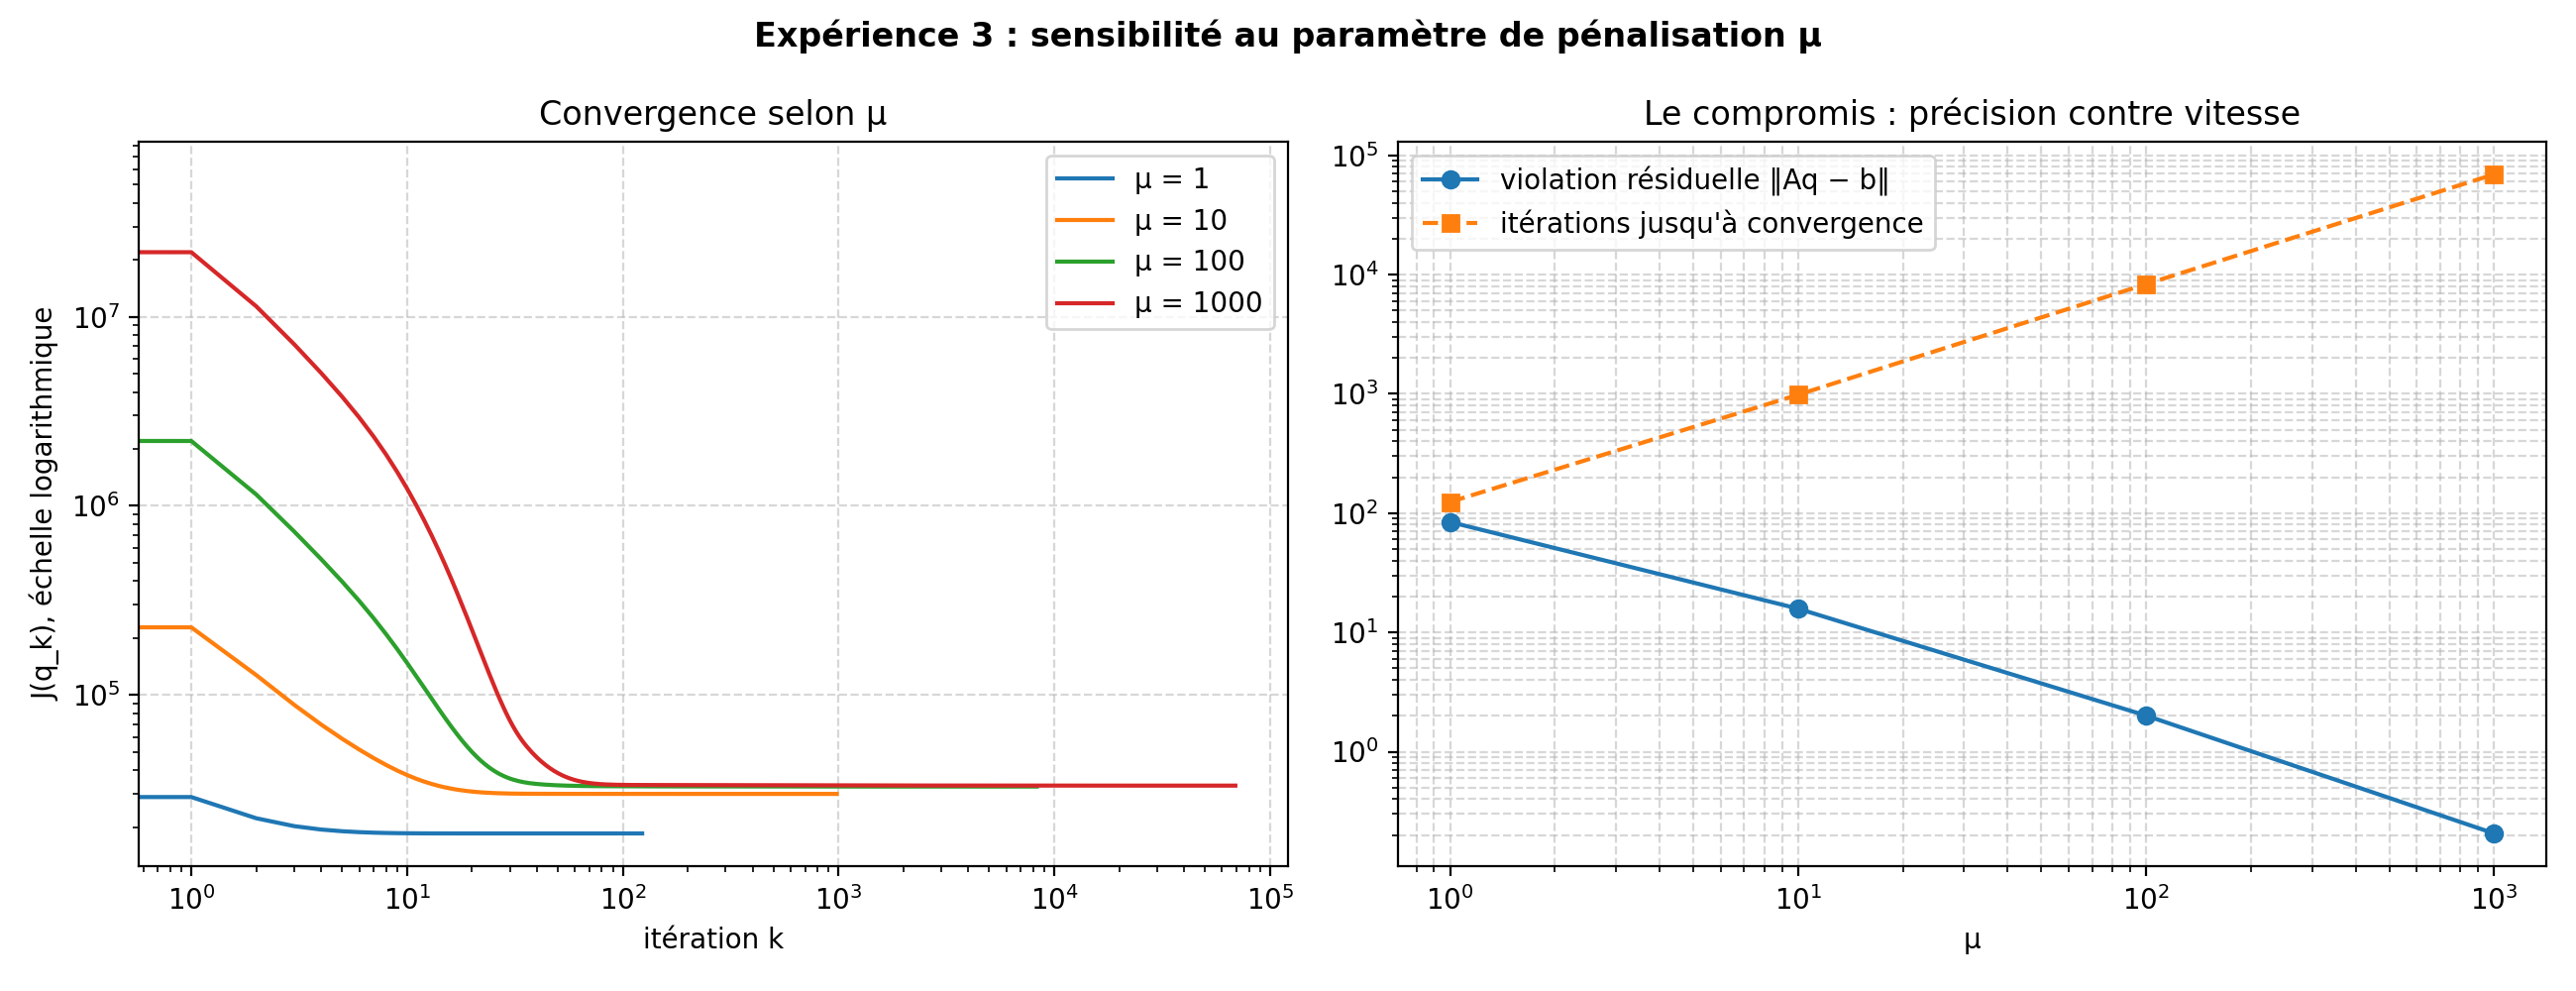
\includegraphics[width=0.88\textwidth]{../results/figures/exp3_sensibilite_mu.png}
\caption{Sensibilité de la résolution au paramètre de pénalisation $\mu$.}
\label{fig:exp3}
\end{figure}

\begin{figure}[htbp]
\centering
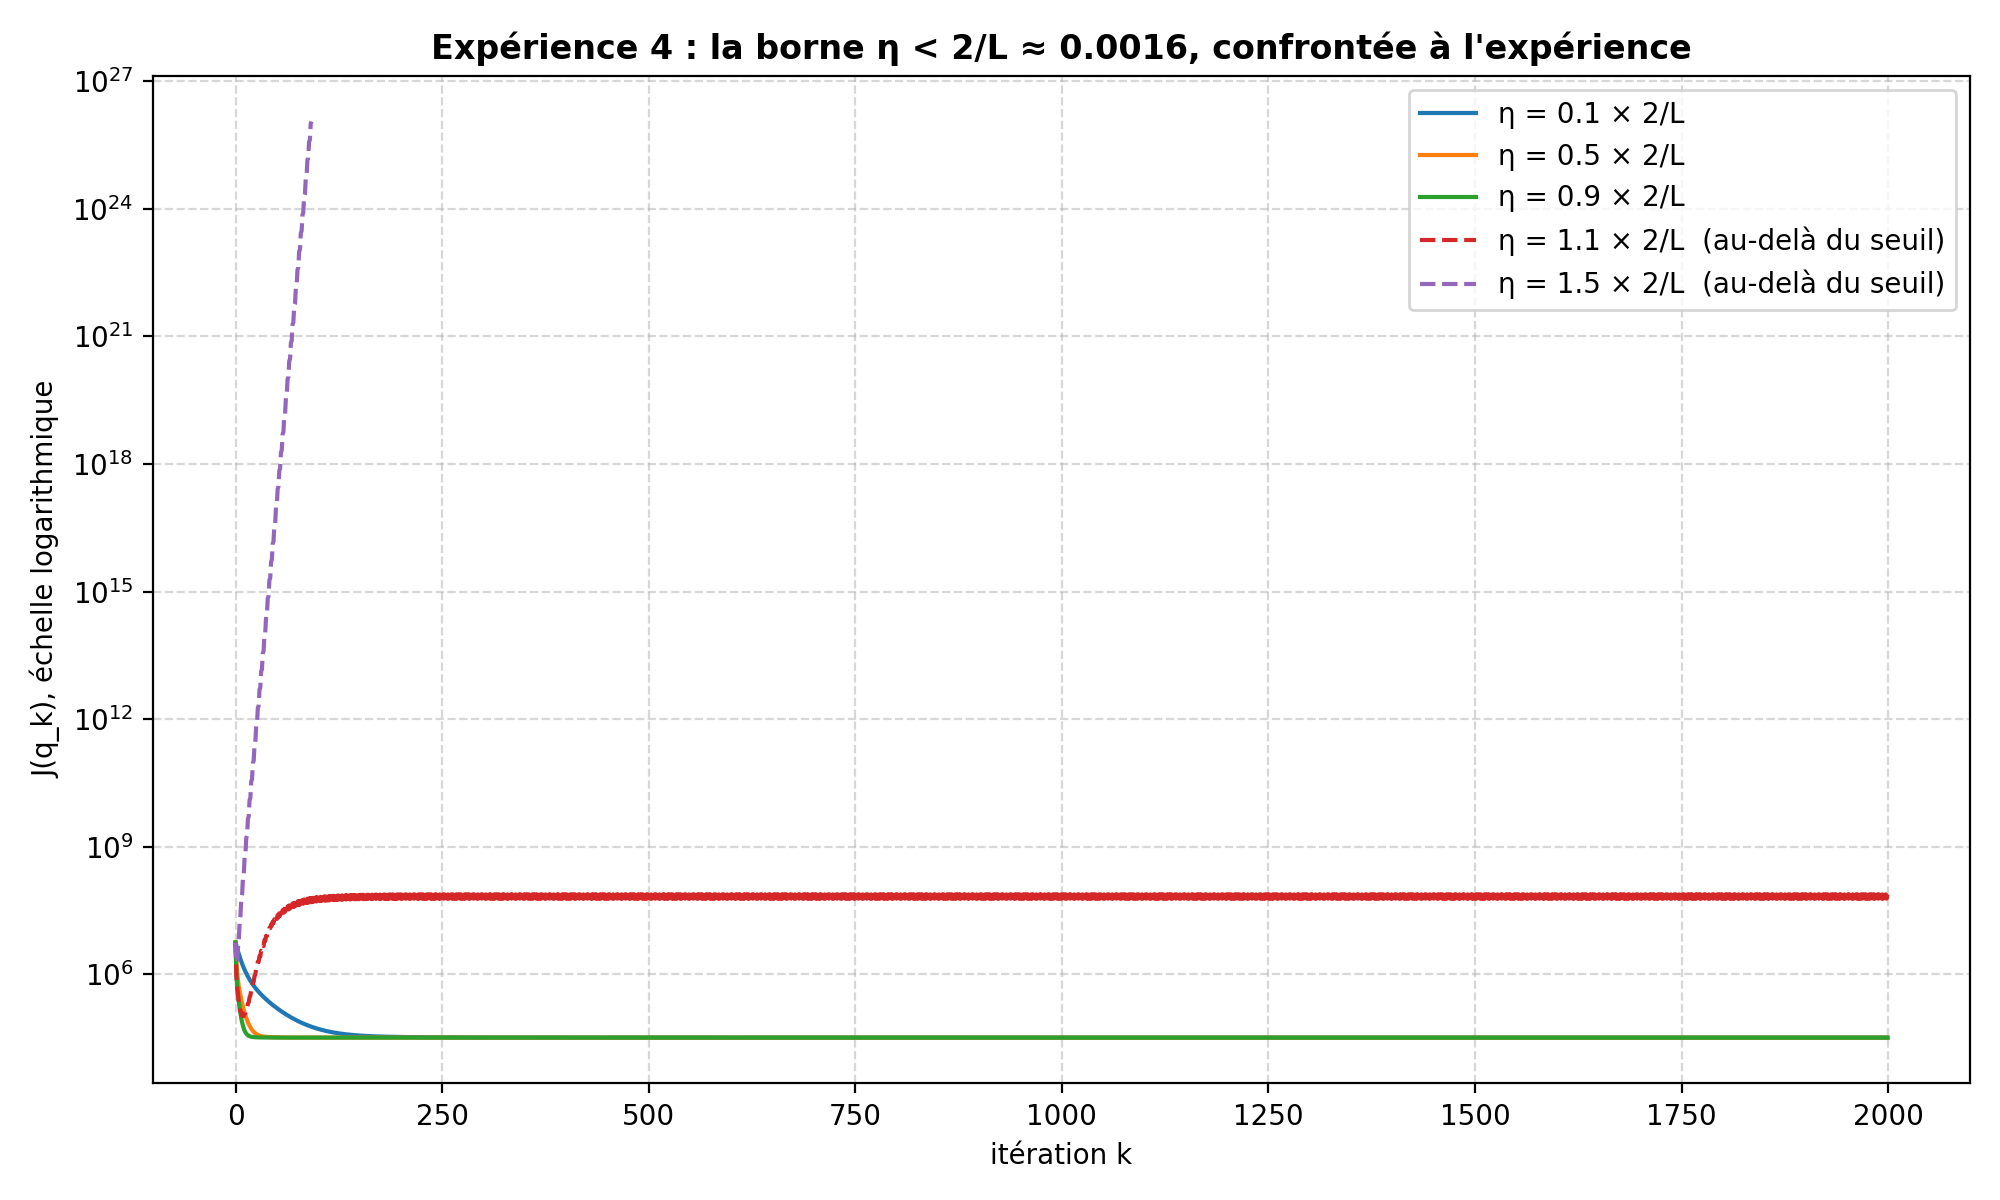
\includegraphics[width=0.88\textwidth]{../results/figures/exp4_convergence.png}
\caption{Confrontation expérimentale à la borne théorique $\eta<2/L$.}
\label{fig:exp4}
\end{figure}

\begin{figure}[htbp]
\centering
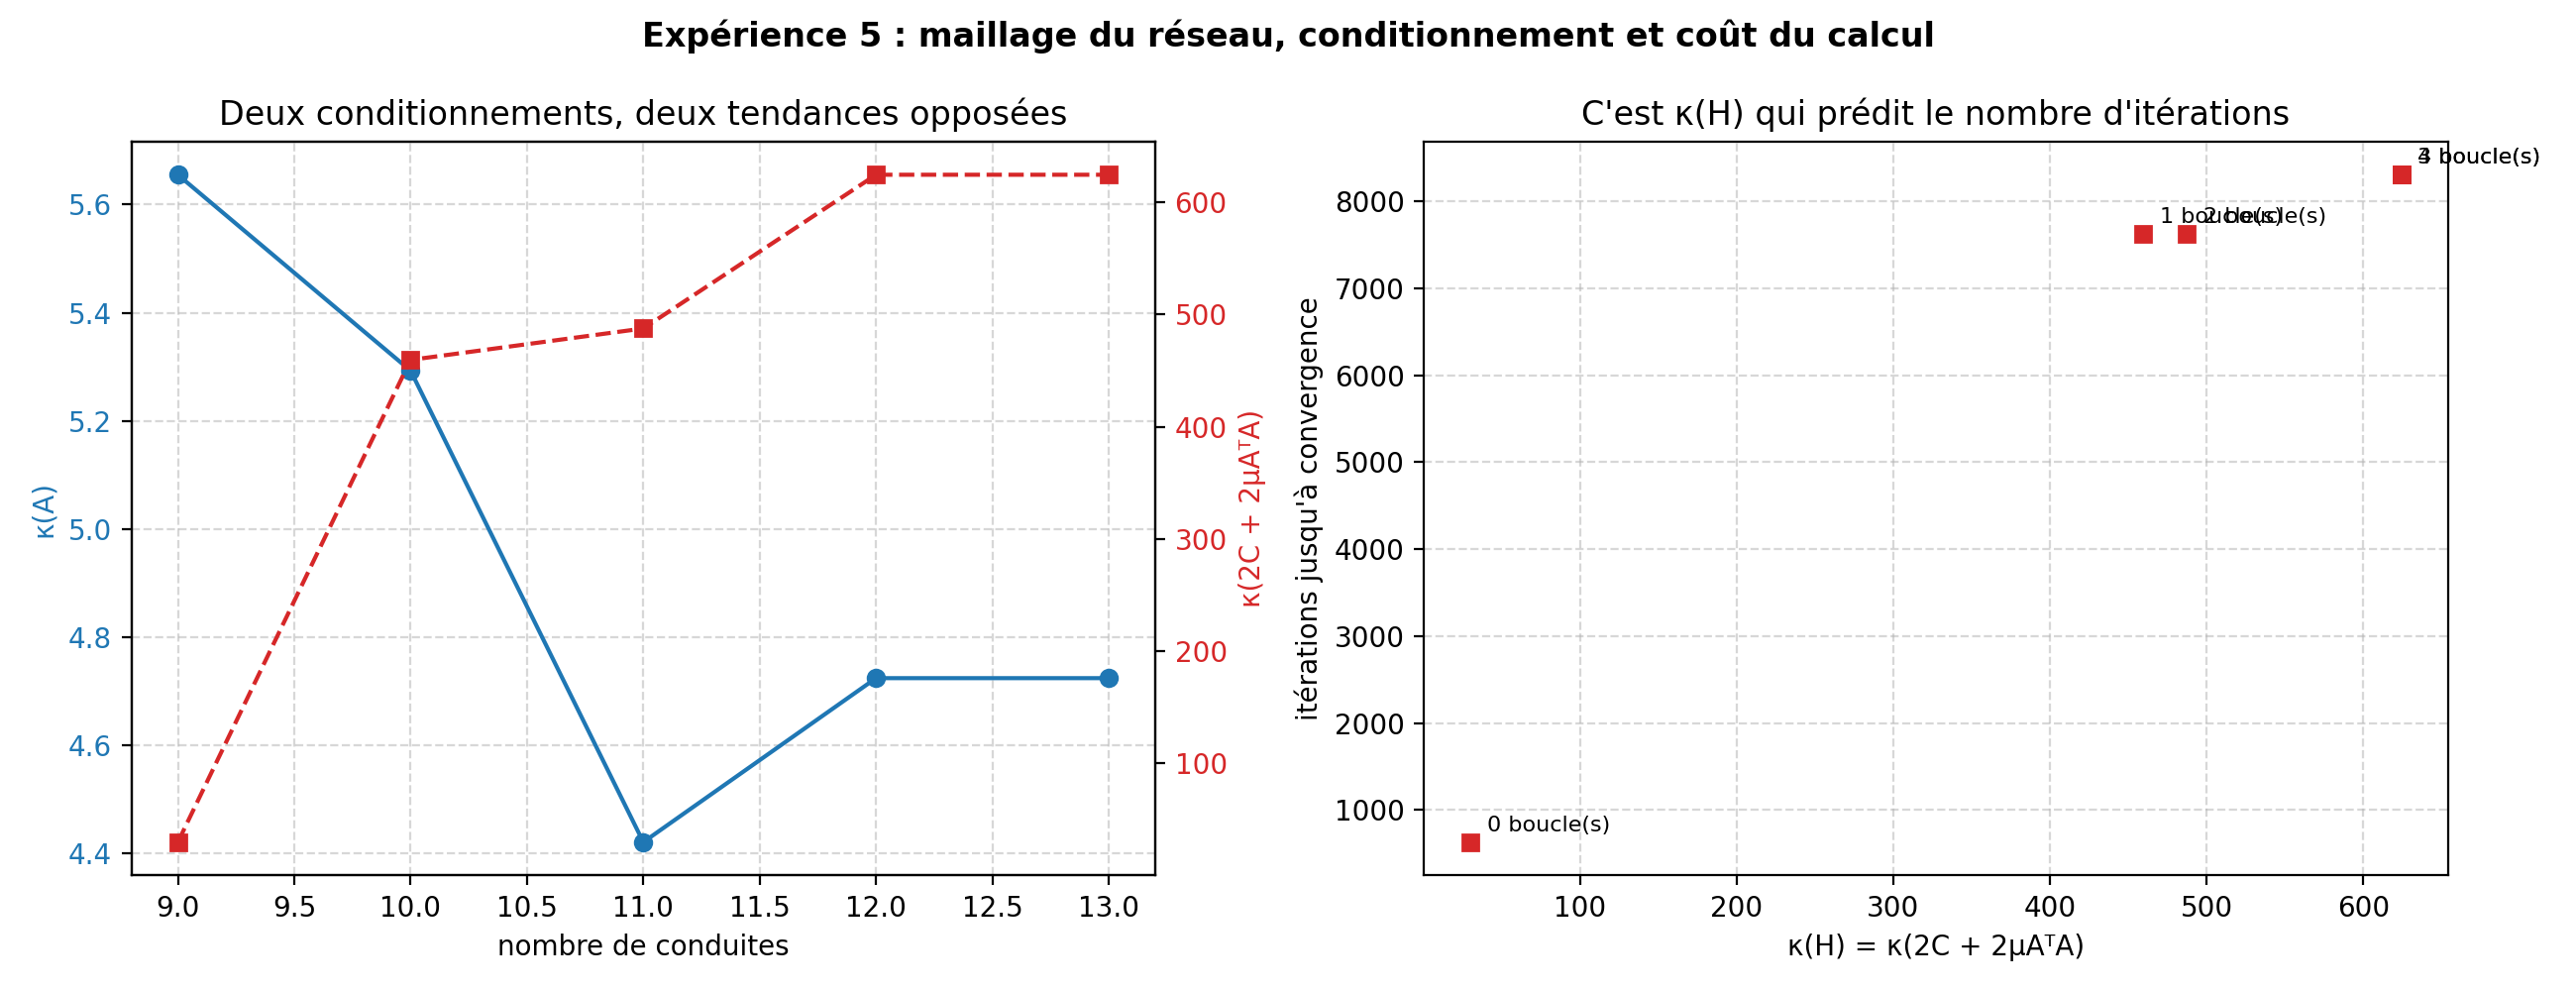
\includegraphics[width=0.88\textwidth]{../results/figures/exp5_maillage_conditionnement.png}
\caption{Effet de la densité du réseau sur le conditionnement et la convergence.}
\label{fig:exp5}
\end{figure}

L'Expérience~6 fournit en outre quatre figures sur les corrélations, les densités de demande,
la convergence de la moyenne empirique et le profil de risque des quartiers.

\begin{figure}[htbp]
\centering
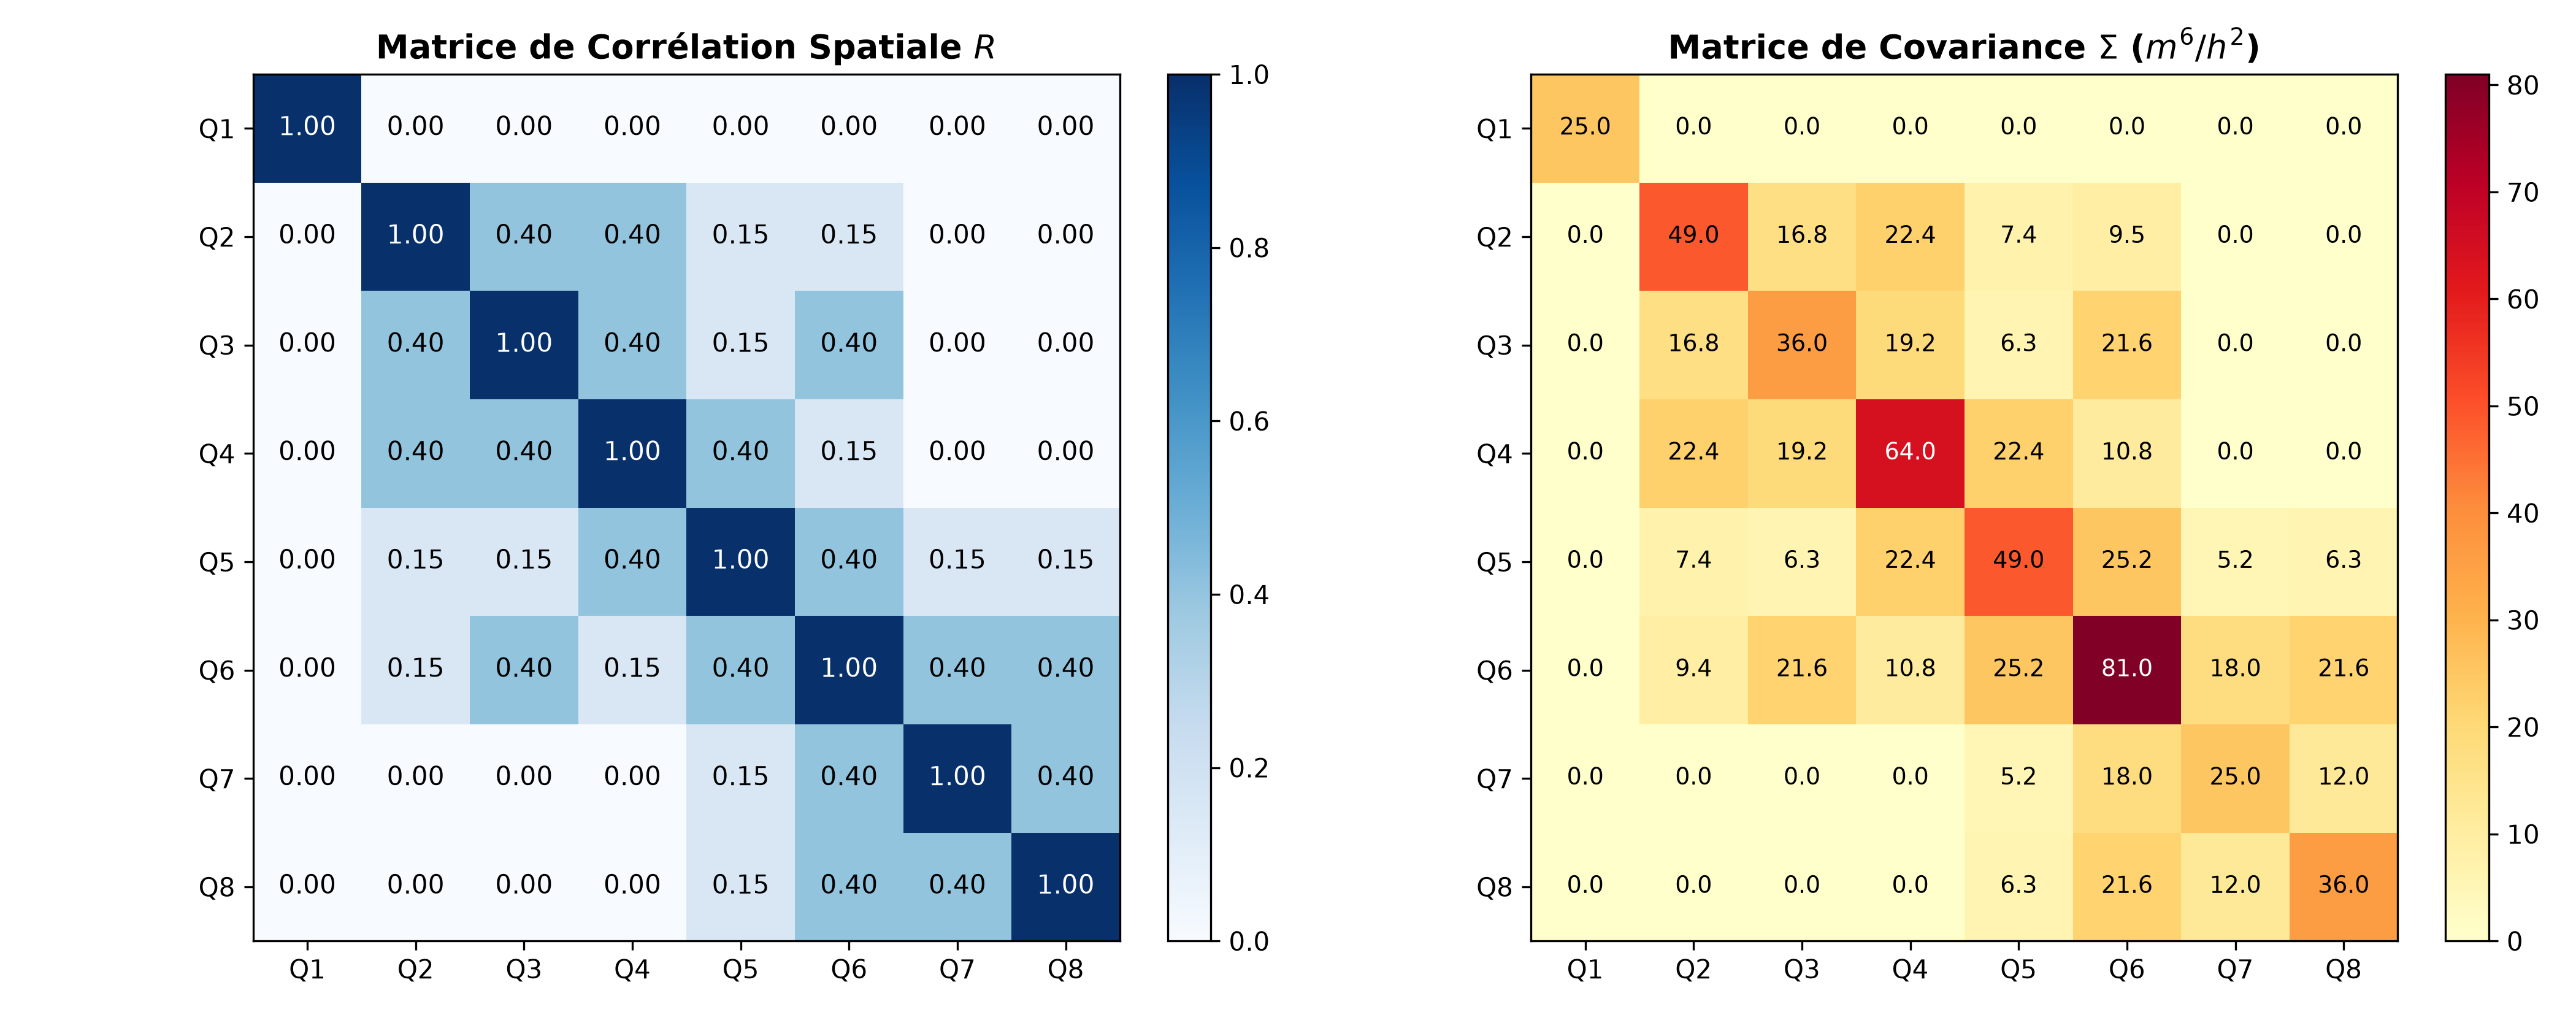
\includegraphics[width=0.88\textwidth]{../results/figures/fig1_matrices_correlation_covariance.png}
\caption{Corrélations et covariance simulées entre quartiers.}
\label{fig:exp6-correlation}
\end{figure}

\begin{figure}[htbp]
\centering
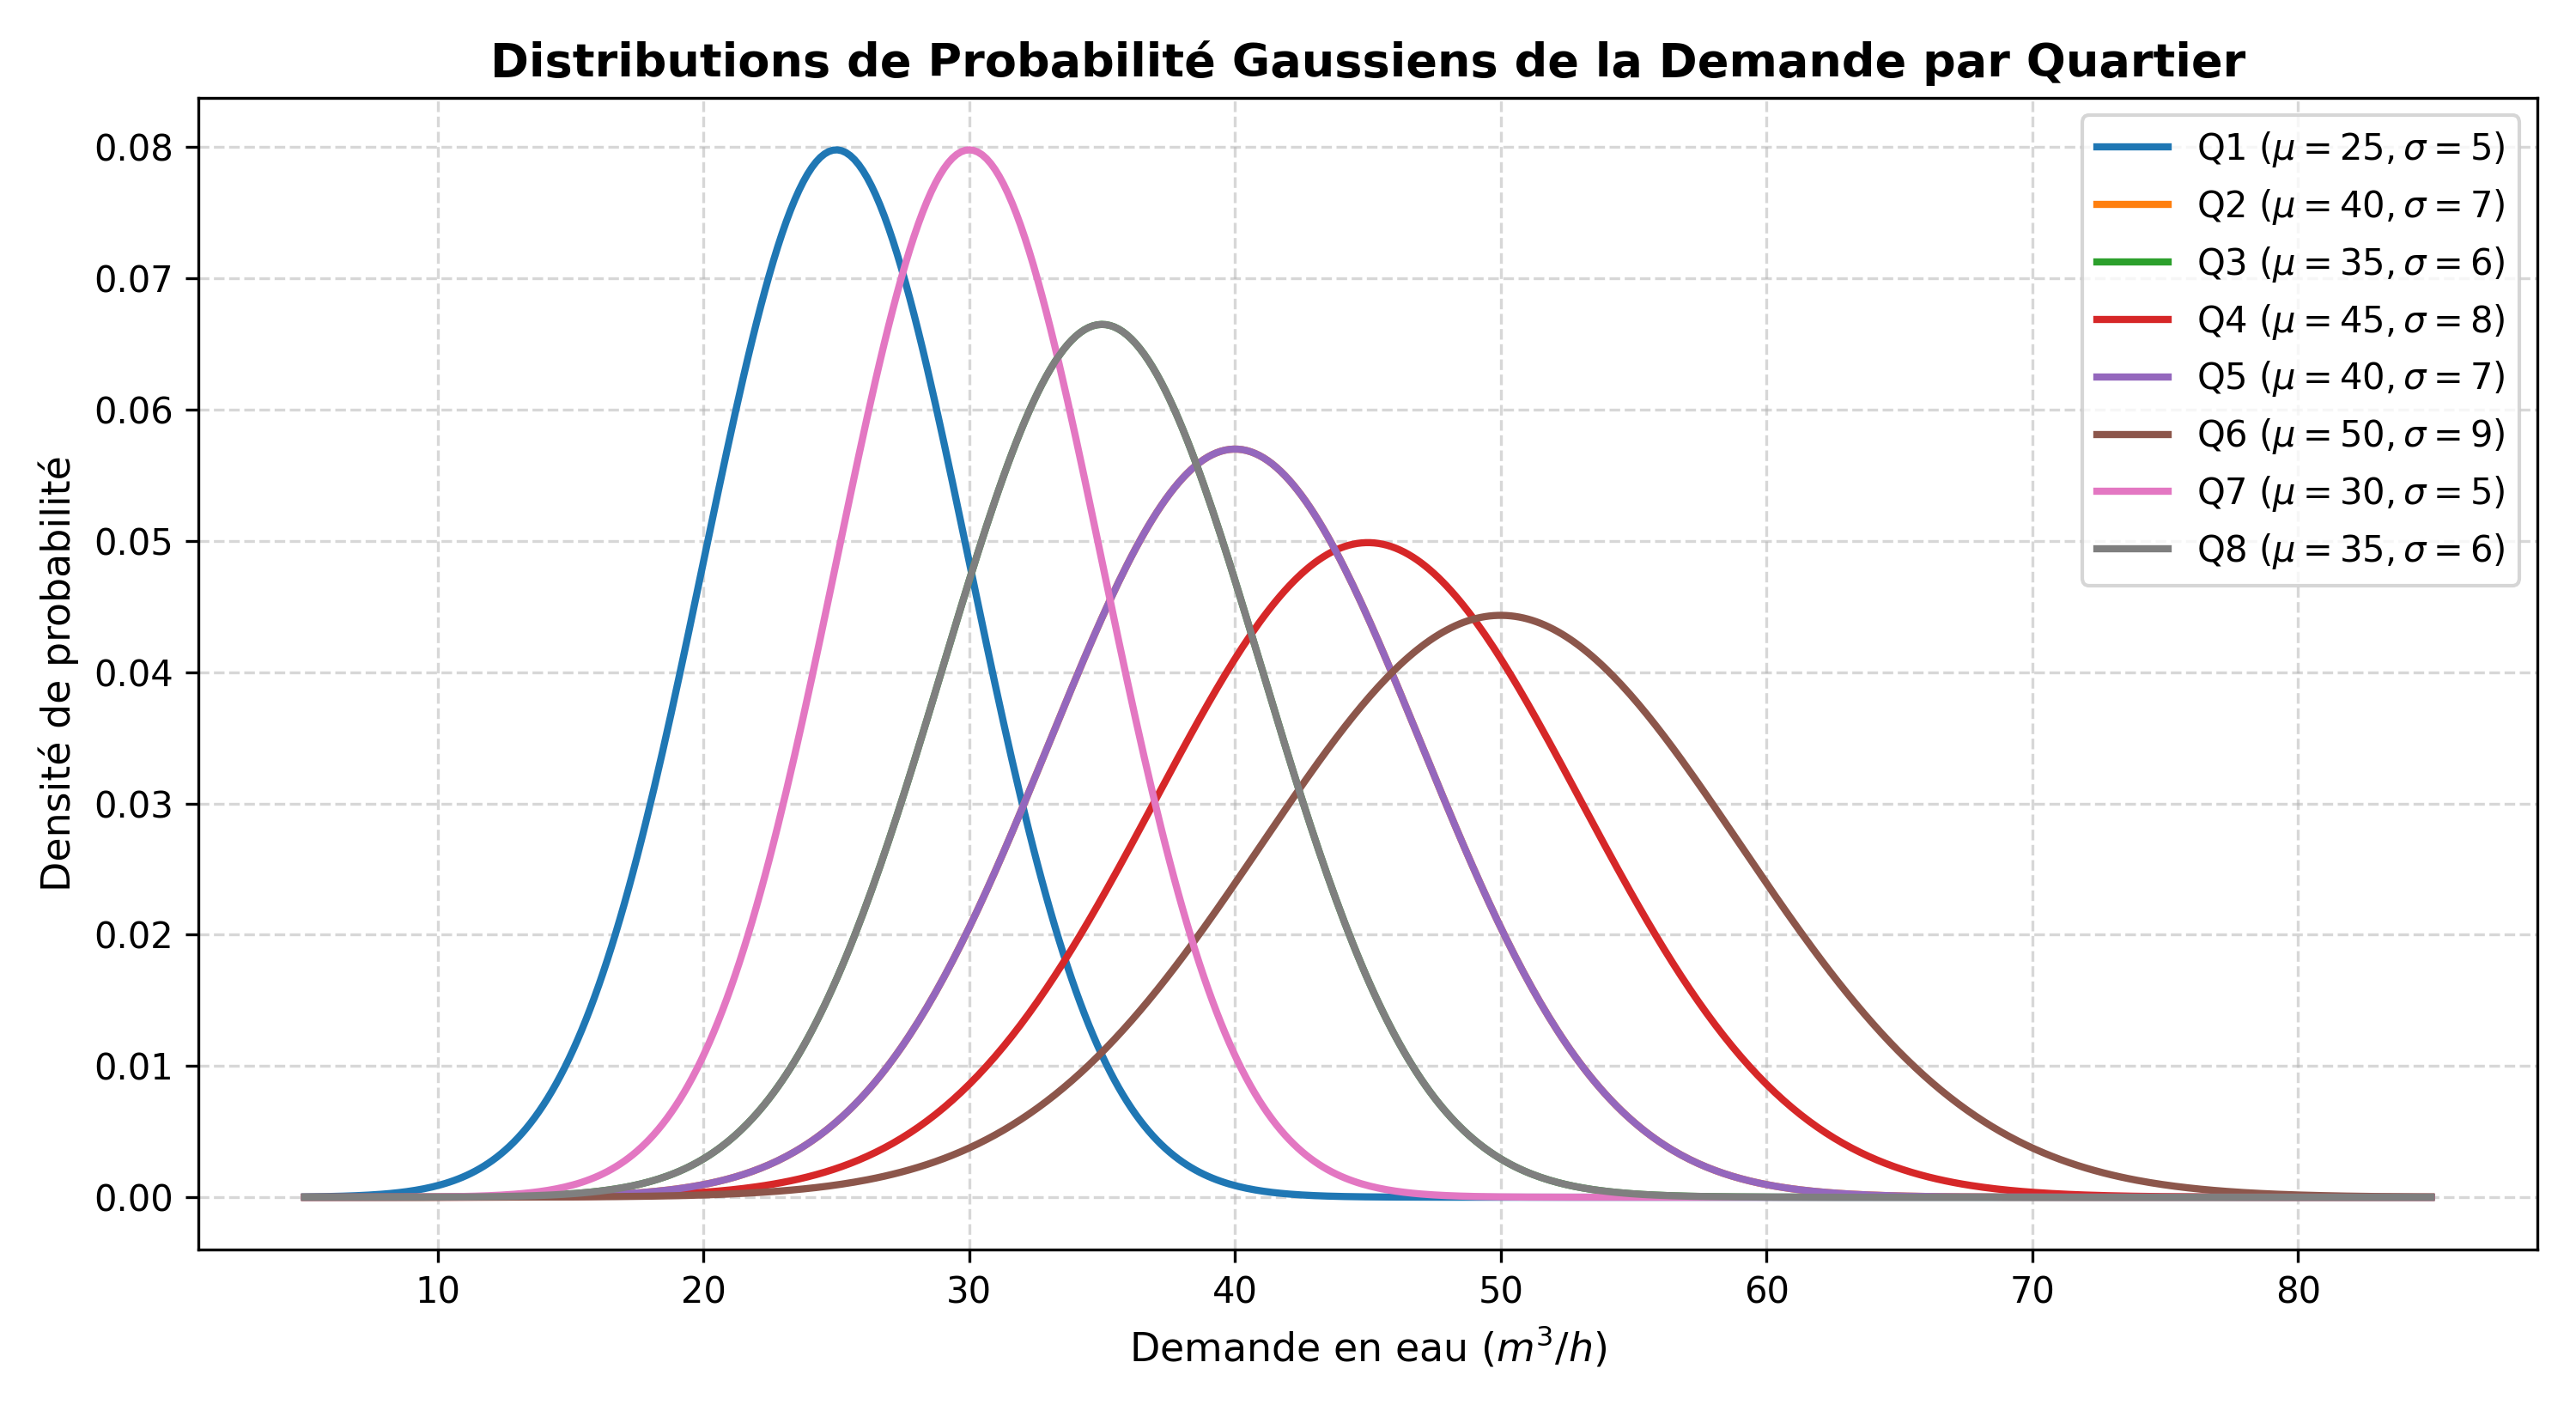
\includegraphics[width=0.88\textwidth]{../results/figures/fig2_densites_probabilites_demande.png}
\caption{Densités empiriques des demandes simulées.}
\label{fig:exp6-densites}
\end{figure}

\begin{figure}[htbp]
\centering
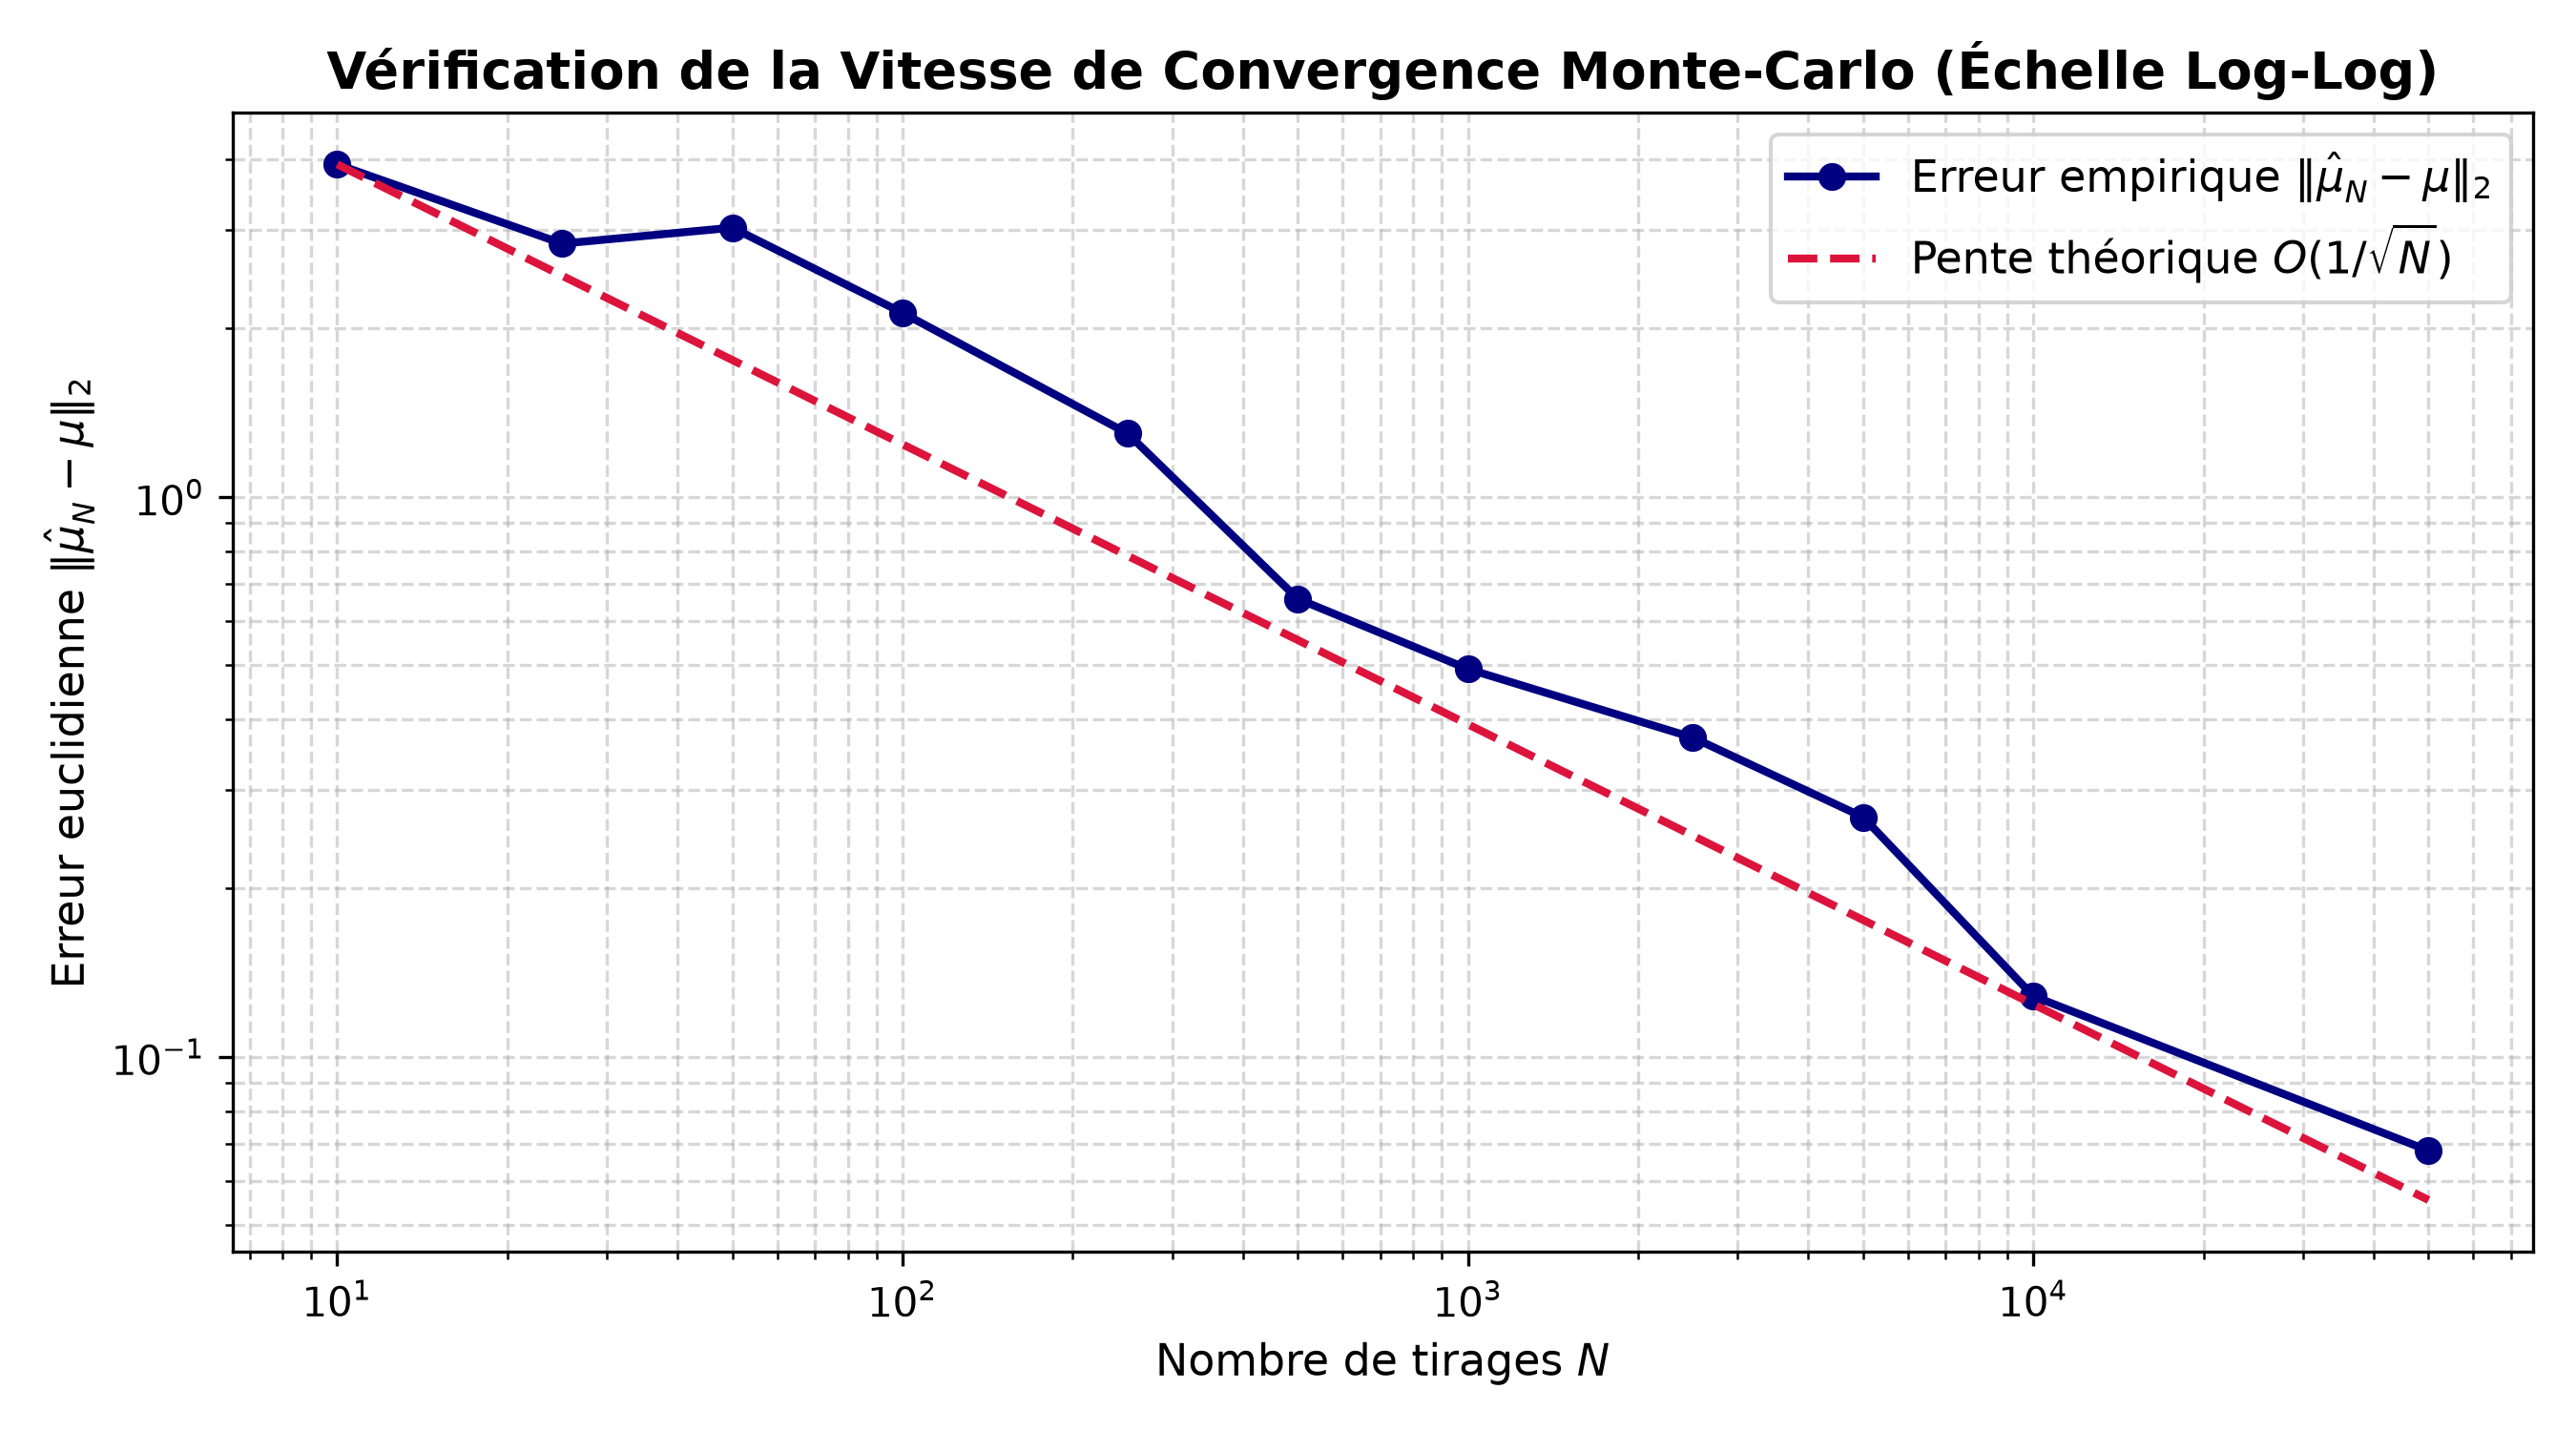
\includegraphics[width=0.88\textwidth]{../results/figures/fig3_convergence_loi_grands_nombres.png}
\caption{Convergence de la moyenne empirique et erreur d'estimation.}
\label{fig:exp6-convergence}
\end{figure}

\begin{figure}[htbp]
\centering
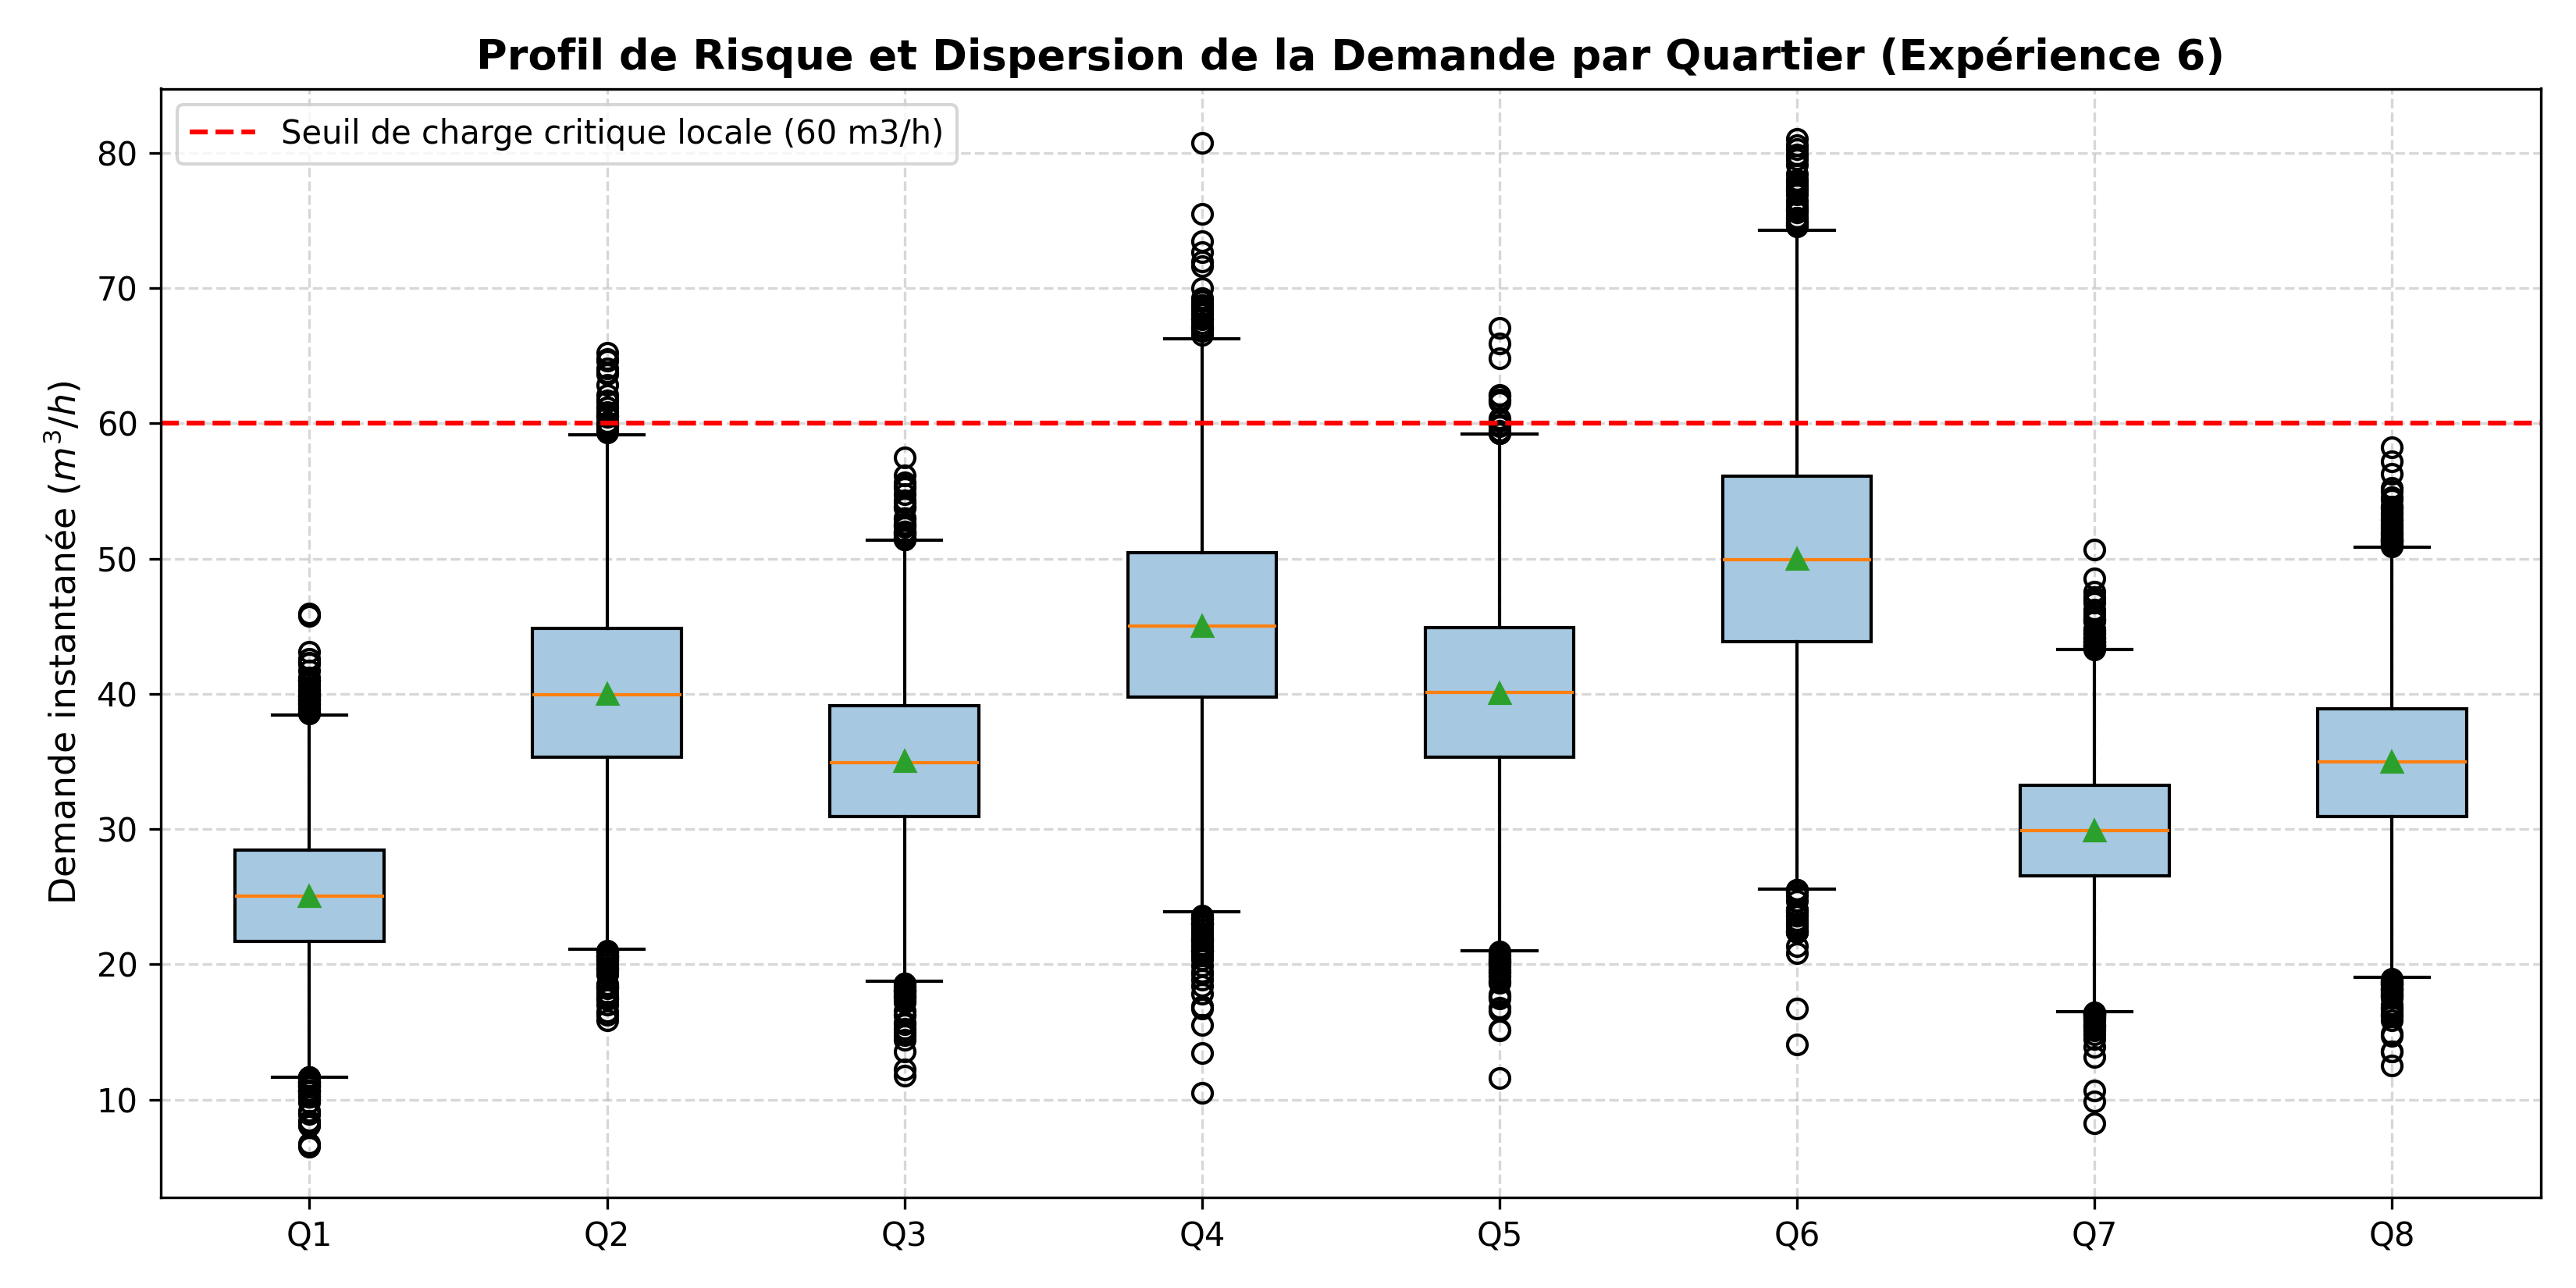
\includegraphics[width=0.88\textwidth]{../results/figures/fig4_profil_risque_quartiers.png}
\caption{Profil de risque simulé par quartier.}
\label{fig:exp6-risque}
\end{figure}

% =======================================================================
\section{Analyse des résultats}
\label{sec:analyse}
% =======================================================================

Les sorties confirment le rôle de la Hessienne : augmenter $\mu$ réduit fortement le résidu,
mais augmente $L$ et le nombre d'itérations. La borne $2/L$ est également observée
expérimentalement. Le maillage ne doit pas être interprété uniquement par son nombre d'arêtes,
car la stabilité dépend de la combinaison $(A,C,\mu)$.

La comparaison à la référence montre un gain de coût moyen de $4{,}83\,\%$ et un effet
statistiquement très significatif. Elle ne démontre pas une supériorité universelle : la
référence satisfait exactement chaque demande quartier par quartier, tandis que la solution
pénalisée accepte une petite violation pour réduire le coût. L'équité doit donc être évaluée
avec les taux de satisfaction et non déduite du seul coût technique.

% =======================================================================
\section{Limites et améliorations possibles}
\label{sec:limites}
% =======================================================================

\begin{itemize}[leftmargin=*]
    \item \textbf{Ponts non redondés.} Les conduites $R_1\!-\!Q_1$ et $R_1\!-\!Q_2$ restent des
    points de fragilité assumés : toute panne sur l'une d'elles isole une partie du réseau,
    sans alternative possible dans la topologie retenue.
    \item \textbf{Orientation figée des conduites.} Imposer $q_e\ge 0$ sur l'orientation de
    référence des boucles et connexions inter-zones interdit au solveur d'inverser le sens de
    circulation, alors que rien ne l'exclut physiquement.
    \item \textbf{Modèle gaussien de la demande.} La loi normale autorise, en théorie, des
    valeurs de demande négatives, même si cet événement reste rare compte tenu des écarts-types
    retenus (15 à 20\,\% de la moyenne).
    \item \textbf{Redondance $N-1$ partielle.} Les boucles de secours ne couvrent que la
    demande du quartier directement accessible par le chemin alternatif, et non celle de
    l'ensemble d'une branche principale.
    \item \textbf{Capacités non imposées dans l'optimisation.} Les dépassements éventuels sont
    contrôlés a posteriori mais ne sont pas intégrés comme contraintes actives.
\end{itemize}

% =======================================================================
\section{Conclusion}
% =======================================================================

La structure discrète, l'algèbre linéaire, le modèle probabiliste et la dérivation de
l'optimisation sont établis. Les six expériences valident le rôle de $\mu$, la borne de pas,
les effets du maillage, l'analyse statistique des demandes et la comparaison à la référence.
Sur les données synthétiques étudiées, $q^\star$ réduit le coût technique d'environ $4{,}83\,\%$
en moyenne avec un effet statistiquement significatif. Cette conclusion reste conditionnée au
modèle gaussien tronqué, à l'orientation fixée et à l'absence de contraintes de capacité dans
le solveur.

% =======================================================================
\renewcommand{\refname}{Références bibliographiques}
\begin{thebibliography}{99}
\makeatletter
\def\@openbib@code{\itemsep=0.35em\parsep=0pt}
\makeatother

\bibitem{sujets-ama}
Ir.~Charbel Mamlankou, \emph{Thèmes de recherche appliquée}, document de sujets, Académie des
Mathématiques Appliquées (AMA), 2026.

\bibitem{cours}
Ir.~Charbel Mamlankou, \emph{Mathématiques fondamentales pour l'IA}, support de cours, AMA,
2026.

\bibitem{web-incidence}
Wikipédia, \emph{Matrice d'incidence}. \href{https://fr.wikipedia.org/wiki/Matrice_d'incidence}{[Article en ligne]}.

\bibitem{video-graphes}
Ressources audiovisuelles sur les matrices d'incidence et connexité :
\href{https://www.youtube.com/watch?v=c1m7L_fHLXU}{Tutoriel d'introduction} et
\href{https://www.youtube.com/watch?v=PMWo9xweSEA}{Graphes et matrices d'incidence}.

\bibitem{claude}
Anthropic, \emph{Claude} [Grand modèle de langage], 2026. Disponible sur :
\url{https://www.anthropic.com/claude}.
\end{thebibliography}

% =======================================================================
\appendix
\section{Résultats d'exécution du code et visualisation du graphe}
\label{sec:annexes-executions}
% =======================================================================

Cette annexe regroupe les sorties effectives des modules d'implémentation, validant
numériquement l'ensemble des théorèmes et propriétés topologiques établis dans le rapport.

\subsection{Validation de la construction matricielle (\texttt{build\_graph.py})}

La commande \texttt{python3 -m src.graph.build\_graph} instancie le graphe orienté ($n=10$,
$m=13$), assemble la matrice d'incidence $A\in\mathbb{R}^{10\times 13}$ ainsi que le vecteur de
coût $c_e$ et le second membre $b$.

\begin{figure}[htbp]
\centering
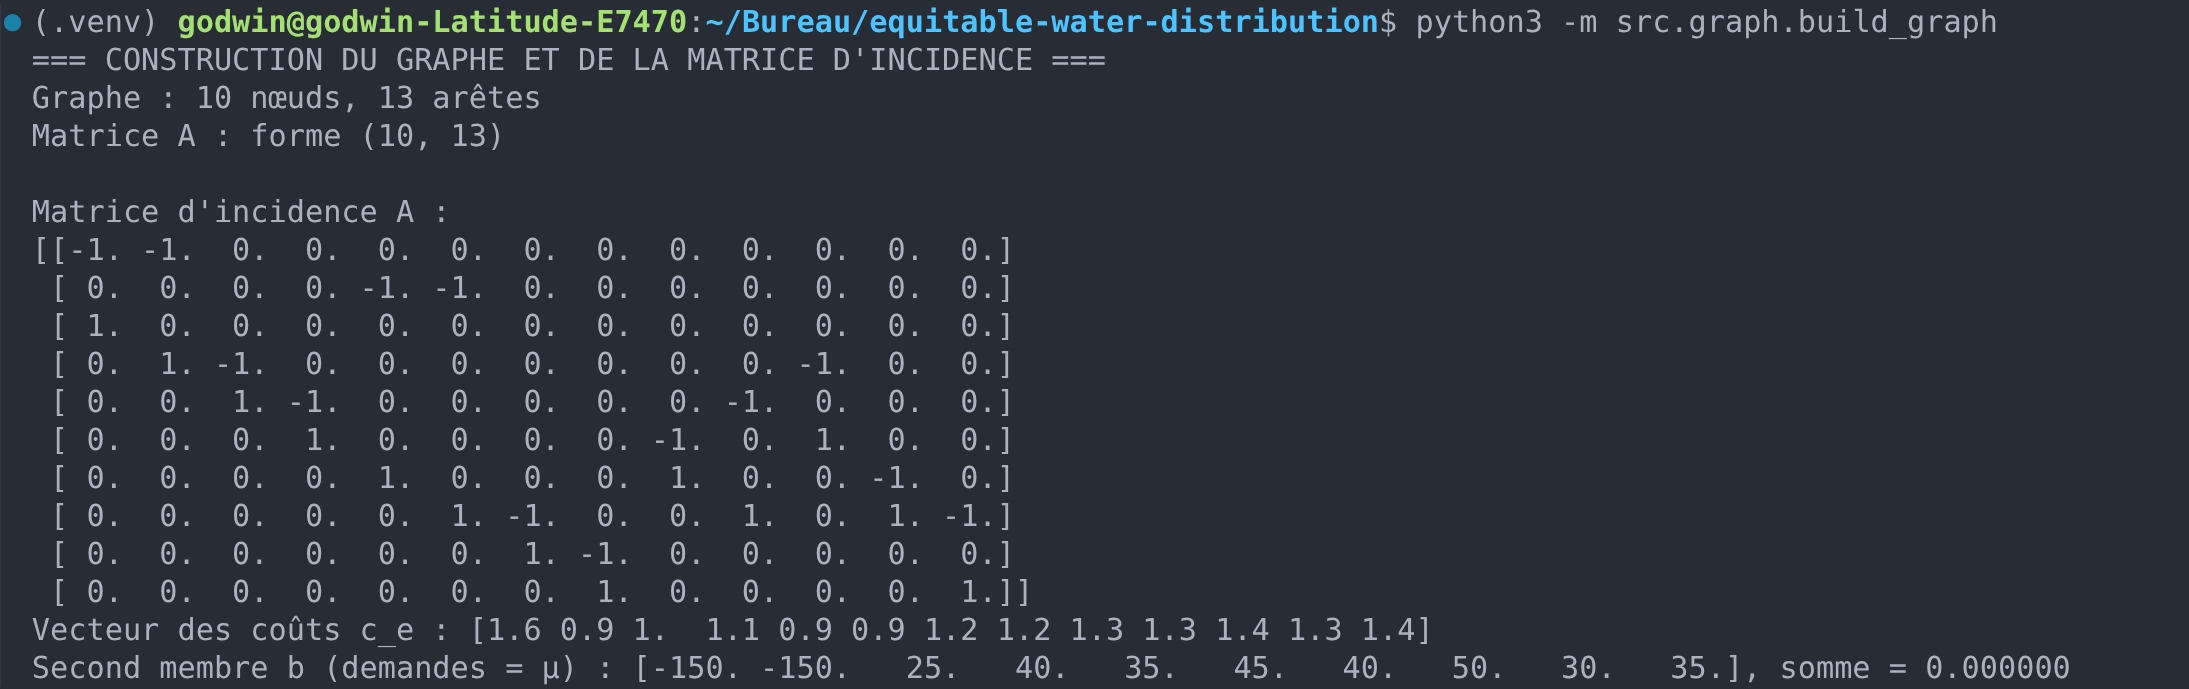
\includegraphics[width=\textwidth]{../docs/algebre_lineaire/capture_build_graph.png}
\caption{Sortie terminal confirmant la structure de la matrice d'incidence $A$, le vecteur des
coûts $c_e$ et la conservation globale $\sum b_i=0$.}
\label{fig:exec-build}
\end{figure}

\subsection{Analyse spectrale et points de fragilité (\texttt{graph\_analysis.py})}

L'exécution du script \texttt{src.graph.graph\_analysis} corrobore l'ensemble des grandeurs
théoriques : rang effectif $\operatorname{rg}(A)=9$, dimension du noyau $\dim\ker(A)=4$,
conditionnement $\kappa(A)\approx 4{,}7244$, constante de Lipschitz
$L(\mu{=}1{,}0)\approx 14{,}9525$, ainsi que la détection exacte des ponts et points
d'articulation.

\begin{figure}[htbp]
\centering
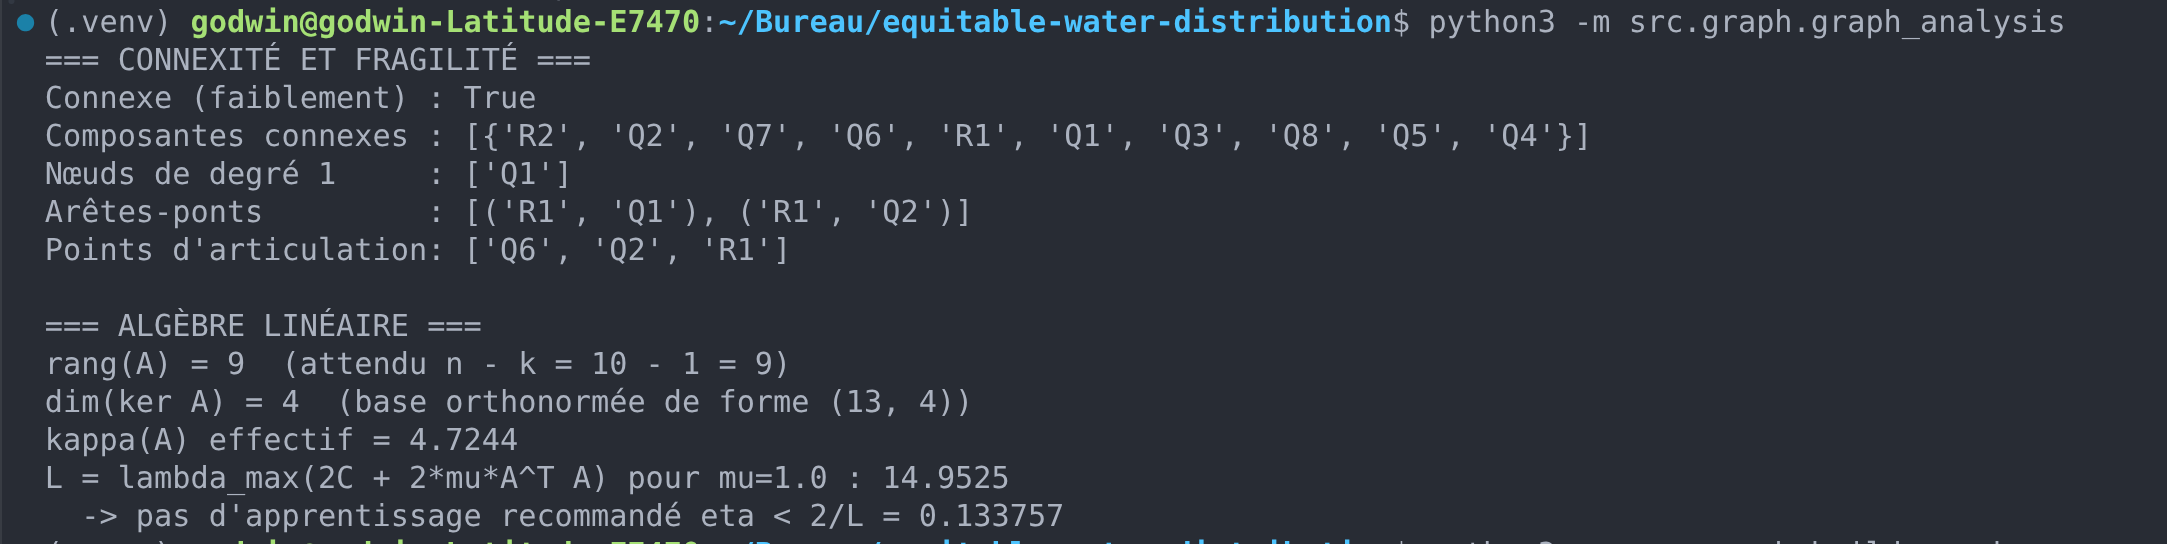
\includegraphics[width=\textwidth]{../docs/algebre_lineaire/capture_analysis.png}
\caption{Validation numérique de la connexité, des points de fragilité, du rang, du
conditionnement effectif et de la borne de Lipschitz $\eta<0{,}133757$.}
\label{fig:exec-analysis}
\end{figure}

\clearpage
\subsection{Visualisation spatiale du réseau de distribution}

\begin{figure}[htbp]
\centering
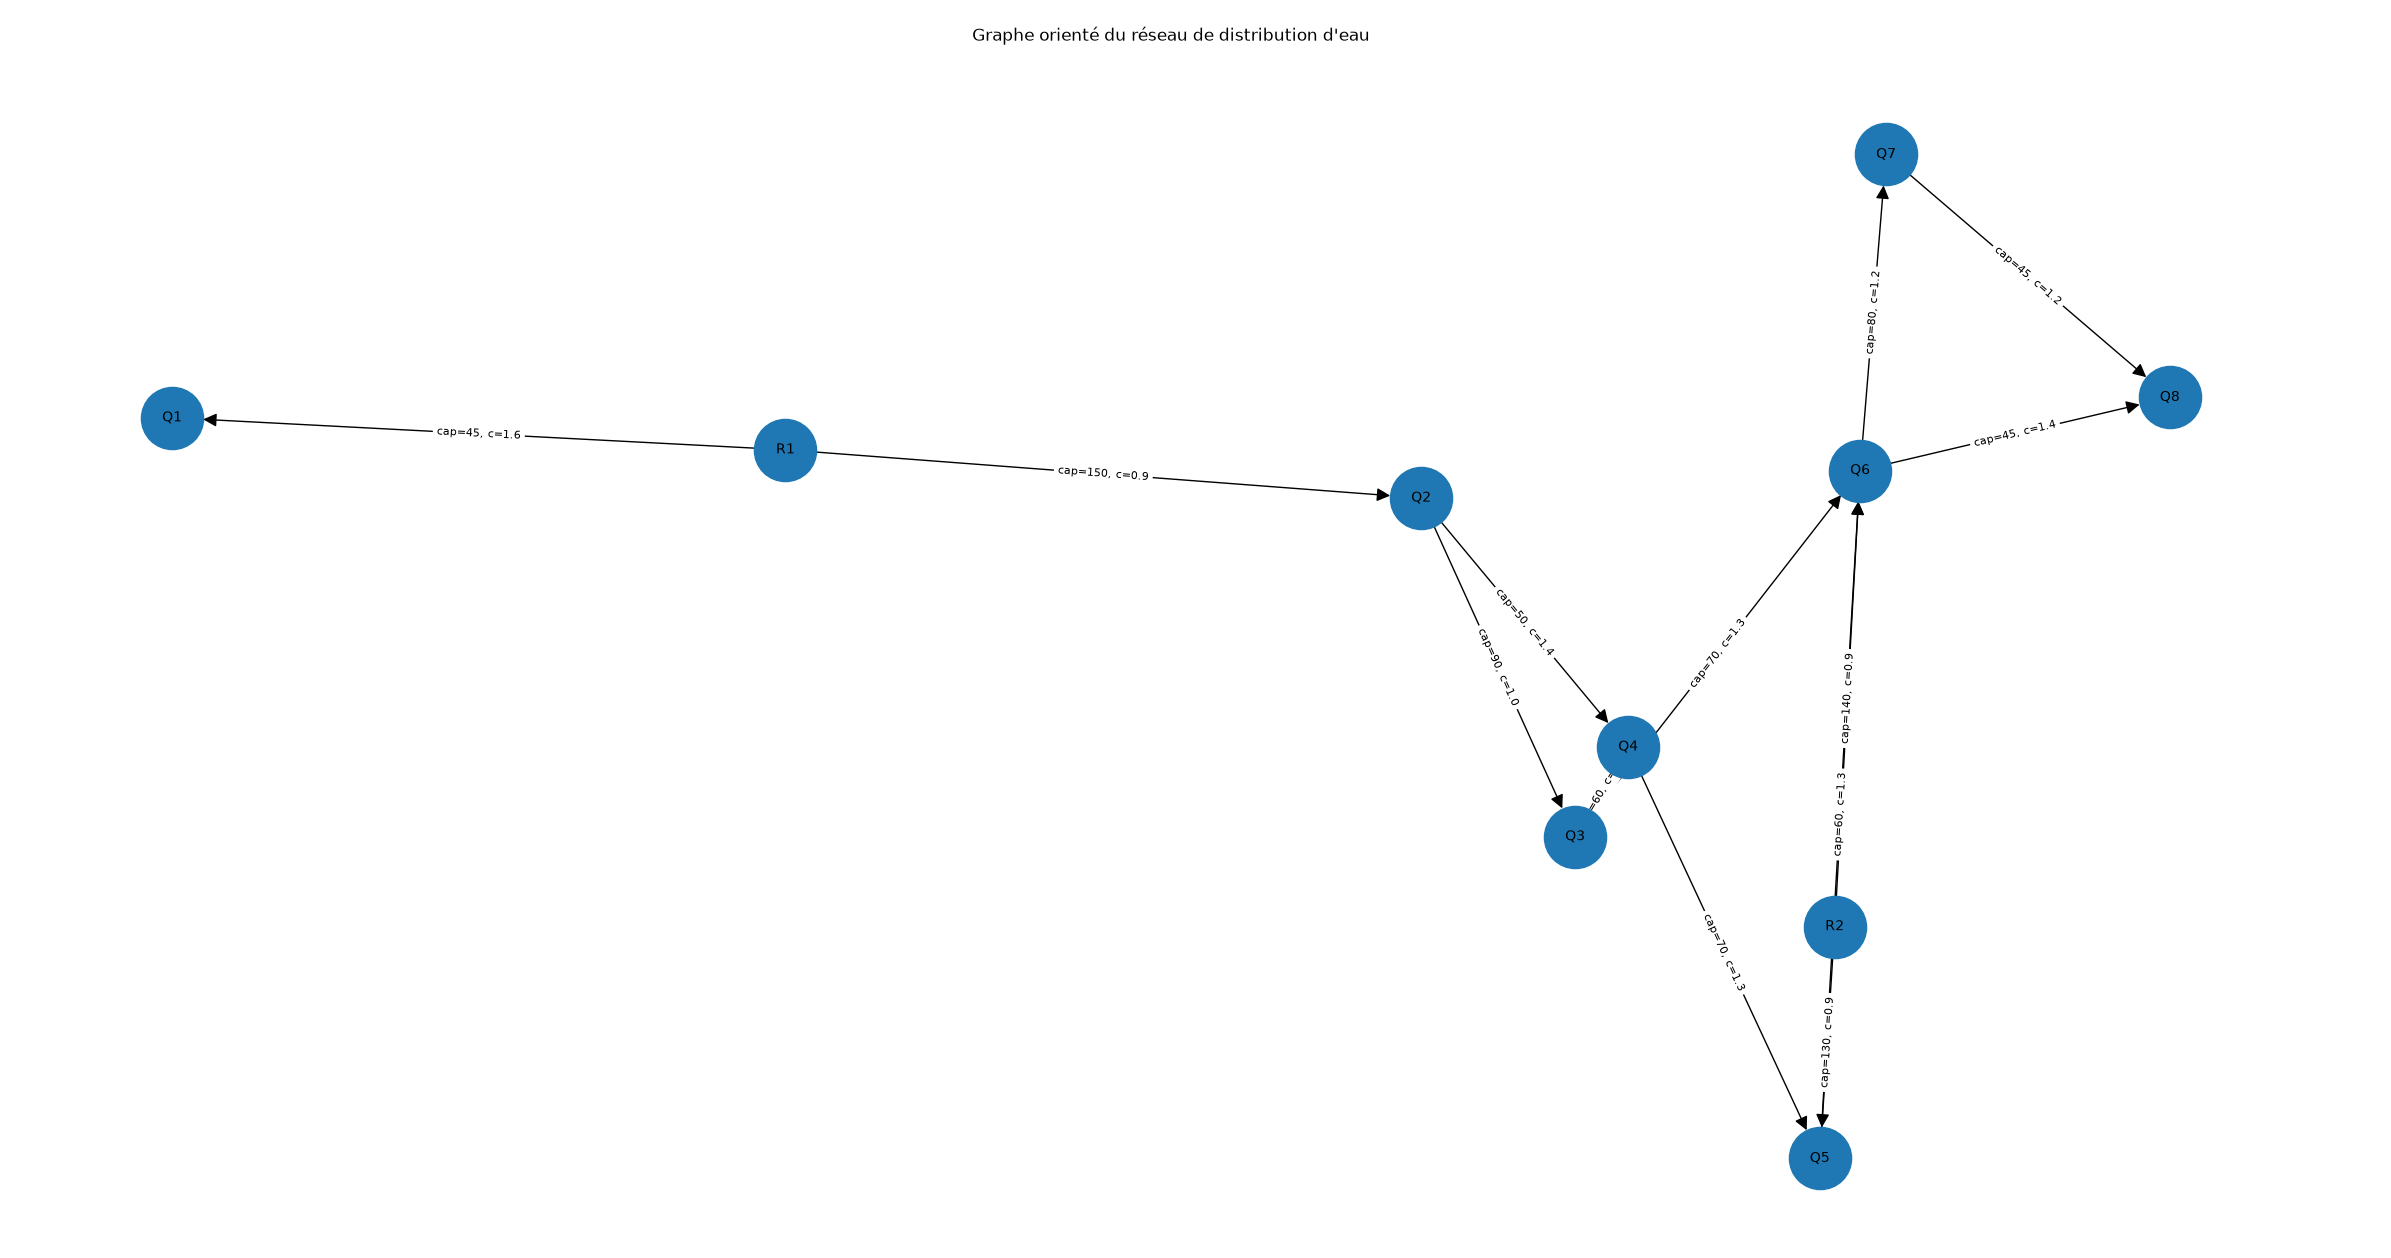
\includegraphics[width=\textwidth, trim={4cm 1cm 4cm 1cm}, clip]{../docs/algebre_lineaire/graphe_reseau.png}
\caption{Représentation topologique orientée du réseau d'eau, illustrant les réservoirs
$\{R_1,R_2\}$, les quartiers $\{Q_1,\dots,Q_8\}$, les arêtes-ponts vers $Q_1$ et la redondance
maillée de la zone aval.}
\label{fig:topologie-visuelle}
\end{figure}

\end{document}
